\documentclass[preprint,review,12pt,3p]{elsarticle}
\usepackage[utf8]{inputenc}
\usepackage{hyperref}
\hypersetup{hidelinks}
\usepackage{doi}
\usepackage{amssymb}
\usepackage{amsmath}
\usepackage{lineno}
\linenumbers
\usepackage{graphicx}
\usepackage{float}
\usepackage{caption}
\usepackage{subcaption}
\usepackage{amsthm}
\usepackage{booktabs}
\usepackage{array}
\usepackage{multirow}
\usepackage{tikz}
\usetikzlibrary{arrows, positioning, shapes}
\usepackage{pgfplots}
\pgfplotsset{compat=1.18}
\usepackage{bbm}
\usepackage{natbib}

\DeclareMathOperator{\E}{\mathbb{E}}
\DeclareMathOperator{\tr}{tr}

\newtheorem{theorem}{Theorem}[section]
\newtheorem{lemma}[theorem]{Lemma}
\newtheorem{corollary}[theorem]{Corollary}

\graphicspath{{figure/}{figure/media/}}

\journal{Ecological Informatics}

\begin{document}
	
	\begin{frontmatter}
		
		\title{A physics-informed framework for ecohydrological parameter inversion and dynamical exploration in the lower Tarim River}
		
		\author{Yingxin Pang}
		\address{School of Mathematics and Statistics, North China University of Water Resources and Electric Power, Zhengzhou, 450046, China}
		
		\author{Jinhua Zhang}
		\address{School of Electrical Engineering, North China University of Water Resources and Electric Power, Zhengzhou, 450046, China}
		
		\author{Jianwei Shen\corref{cor1}}
		\address{School of Mathematics and Statistics, North China University of Water Resources and Electric Power, Zhengzhou, 450046, China}
		
		\cortext[cor1]{Corresponding author}
		\ead{shenjianwei@ncwu.edu.cn}
		
		\begin{abstract}
		Arid riparian ecosystems show strong vegetation--water feedbacks and nonlinear responses to ecological water conveyance. We developed a coupled temporal ecohydrological model for the lower Tarim River and inverted its parameters with a physics-informed neural network (PINN), using annual NDVI, TVDI and conveyance records from 2000 to 2023, with the lower Heihe as a descriptive cross-basin reference. The PINN was calibrated on 2000--2018 and evaluated on two windows outside that range: withheld observations (2019--2020) and trend projections (2021--2023). The calibration-period reconstruction reached $R^2=0.993$, $0.996$ and $0.792$ for NDVI, TVDI and cumulative water transfer (RMSE 0.004, 0.005 and $12.5\times10^{8}$ m$^{3}$); outside the calibration range $R^2$ was negative for all three variables and the RMSE exceeded that of a one-year persistence forecast, so the framework is presented as a parameter-inversion and dynamical-exploration tool rather than a predictive model. The calibrated parameters supported equilibrium and stability analysis. No Hopf bifurcation or validated fold threshold was detected in the investigated range; a reduced normal form was used only to explore qualitative fold-like hysteresis, and a reduced reaction--diffusion system served as an exploratory test of Turing compatibility. A persistence-anchored residual spatial PINN, evaluated on three georeferenced 1.28 km windows on a 10 m grid, reproduced the held-out vegetation and water pattern structure (spectral cosine $\approx0.99$; pixel correlation $0.90$--$0.94$) but not the absolute TVDI level, which we report as pattern-level evidence rather than a spatial forecast.
		\end{abstract}
		
		\begin{keyword}
			Physics-informed neural networks \sep Ecohydrological modelling \sep 
			Populus euphratica \sep Dynamical systems \sep Parameter inversion \sep 
			Turing patterns \sep Ecological water conveyance \sep Tarim River basin
		\end{keyword}
		
	\end{frontmatter}
	
	% ==================== 1. Introduction ====================
	\section{Introduction}
	
	Ecosystems in arid and semi-arid regions are characterized by extreme water scarcity, high climatic variability, and strong vegetation--water feedbacks that govern ecosystem structure and function. The Tarim River basin in northwestern China contains an important naturally distributed \textit{Populus euphratica} riparian forest, which plays a critical role in maintaining regional ecological security and preventing desertification \citep{zhou2020ecolind}. Long-term water diversion and groundwater decline have caused substantial ecological degradation, whereas ecological water conveyance since 2000 has promoted vegetation recovery \citep{chen2010hyp,ma2025response,ye2010ecological}. However, recovery remains spatially heterogeneous, suggesting the possible presence of threshold dynamics and alternative ecosystem states \citep{scheffer2001catastrophic}.
	A key challenge in dryland ecology is to describe vegetation responses to changes in water availability using models that account for nonlinear feedbacks and spatial interactions. Existing vegetation-pattern models have shown that local positive feedbacks and longer-range inhibitory processes can generate bistability, hysteresis, and spatial self-organization \citep{borgogno2009mathematical,rietkerk2008regular,vonhardenberg2001diversity,meron2012pattern}. However, these mechanisms have rarely been integrated with data-constrained parameter estimation for the lower Tarim River ecosystem.
	Physics-informed neural networks (PINNs) integrate observational data with governing equations and can be used for forward simulation and inverse parameter estimation of nonlinear dynamical systems \citep{raissi2019physics,karniadakis2021physics,lu2021deepxde}. However, PINNs may suffer from imbalanced loss terms and optimization-related gradient pathologies, which should be considered when interpreting parameter estimates \citep{wang2021gradient}. Their application to coupled vegetation--water dynamics in arid riparian ecosystems remains limited.
Comparable water-limited riparian systems elsewhere in the same arid belt provide a natural reference for interpreting a single-basin calibration. The lower Heihe (Ejina Oasis) is a second terminal-lake oasis that has also received ecological water conveyance since 2000, and it is used here as a descriptive cross-basin reference processed with the same remote-sensing workflow rather than as an independent calibration target.
	
	In this study, we present a physics-constrained framework for parameter inversion and dynamical-system exploration under sparse annual ecological observations. The core is a coupled temporal ecohydrological dynamical system described by nonlinear ordinary differential equations that represent feedbacks among vegetation condition, water stress and ecological water input, embedded as dynamic constraints in a time-dependent PINN. The contributions are organised as follows.

\begin{enumerate}
	\item A coupled temporal vegetation--water--stress model calibrated by a physics-informed neural network, reported with the calibration-period residuals and the spread across independent refits (Section~3.1; Table~\ref{tab:params}).
	\item An evaluation reported in three separate windows, namely calibration, withheld observations and a trend-projection window, together with a comparison against persistence, an AR(1) model and a forward-integrated nonlinear ODE (Section~3.2; Tables~\ref{tab:holdout} and \ref{tab:baseline}).
	\item Equilibrium continuation and a fold and Hopf screen of the full three-dimensional system, followed by a parameter-perturbation audit of that screen (Section~3.3; Fig.~\ref{fig:formal_continuation}; Section~S7).
	\item A reduced cusp normal form used to illustrate possible fold-like hysteresis, and a reduced reaction--diffusion system used to test qualitative compatibility with Turing-type pattern formation (Sections~3.3 and 3.4; Figs.~\ref{fig:bifurcation} and \ref{fig:turing}; Section~S5).
	\item A held-out 10 m pattern test using a persistence-anchored residual spatiotemporal PINN, reported separately from the temporal calibration and restricted to pattern-level vegetation/water validation (Section~3.5; Table~\ref{tab:spatial_pattern}).
	\item A second water-limited basin, the lower Heihe (Ejina Oasis), processed with the same remote-sensing workflow and used as a descriptive cross-basin reference (Section~3.7; Fig.~\ref{fig:cross_basin}; Table~\ref{tab:cross_basin}).
\end{enumerate}

Full implementation details and supplementary results are provided in the Supplementary Material.
	
	% ==================== 2. Model and PINN Framework ====================
	\section{Model and PINN Framework}
	
\subsection{Main Model Formulation}

We represent the annual vegetation--water dynamics using three normalized state variables: vegetation condition $P(t)$, water-stress condition $T(t)$, and water-input state $R(t)$. The variables are scaled to the interval $[0,1]$ during PINN calibration. The normalized ecological-water forcing is denoted by $F(t)$.

The calibrated temporal system is:
\begin{equation}
	\frac{dP}{dt}
	=
	a_1P(1-P)(1-T)+a_2R-a_3TP-a_4P,
	\label{eq:P}
\end{equation}

\begin{equation}
	\frac{dT}{dt}
	=
	b_1(1-P)-b_2R-b_3T,
	\label{eq:T}
\end{equation}

\begin{equation}
	\frac{dR}{dt}
	=
	c_1\left[F(t)-R\right].
	\label{eq:R}
\end{equation}

Here, $a_1$ represents the intrinsic vegetation response, $a_2$ describes the positive contribution of water input to vegetation condition, $a_3$ represents the vegetation--stress interaction, and $a_4$ is the vegetation loss rate. The parameters $b_1$, $b_2$, and $b_3$ describe stress generation, water-related stress reduction, and stress relaxation, respectively. The parameter $c_1$ controls the adjustment of the internal water-input state toward the observed forcing.

The main calibration model is temporal and does not directly solve a spatial reaction--diffusion equation. A separate persistence-anchored spatiotemporal PINN is used only for a held-out 10 m pattern test (Section~\ref{subsec:spatial_pinn}), and a reduced reaction--diffusion system provides a complementary Turing compatibility check (Section~S5).
	
	\subsection{PINN-Based Calibration}
	
	We used a time-dependent PINN with the year $t$ as the only input and $(P,T,R)$ as the three outputs. The network approximates the solution of Eqs.~(\ref{eq:P})--(\ref{eq:R}). The loss function consists of observation, governing-equation, and initial-condition terms:
	
	\begin{equation}
		\mathcal{L}
		=
		\omega_{\mathrm{OBS}}\mathcal{L}_{\mathrm{OBS}}
		+
		\omega_{\mathrm{ODE}}\mathcal{L}_{\mathrm{ODE}}
		+
		\omega_{\mathrm{IC}}\mathcal{L}_{\mathrm{IC}}.
	\end{equation}
	
	In the implementation, the loss weights were
	$\omega_{\mathrm{OBS}}=2$,
	$\omega_{\mathrm{ODE}}=10$, and
	$\omega_{\mathrm{IC}}=5$. The network architecture and optimization procedure are described in Supplementary Section S2.
	\subsection{Data Sources and Preprocessing}
	
	We assembled a 24-year dataset (2000--2023) comprising NDVI, TVDI, a normalized water-input state, and ecological water-conveyance records. NDVI and TVDI were derived from MODIS collections processed in Google Earth Engine. Water-conveyance records were compiled from institutional reports, published assessments and available monitoring documents. The variable-specific processing is described in Supplementary Section S6.
	
	\begin{itemize}
		\item \textbf{NDVI:} Growing-season NDVI was calculated from MODIS MOD13Q1 observations for the lower Tarim River corridor. The index is the normalized difference between near-infrared and red reflectance, following the original remote-sensing formulation \citep{tucker1979red}. The MODIS vegetation-index product specifications are described by Didan~\citep{didan2015mod13q1}. The complete NDVI time series is provided in Supplementary Section S6.
		
		\item \textbf{TVDI:} TVDI was calculated from the NDVI--land surface temperature feature space using MODIS MOD11A2 and MOD13Q1 products. The dry-edge and wet-edge formulation followed the method proposed by Sandholt et al.~\citep{sandholt2002tvdi}. Land-surface-temperature observations were obtained from the MODIS MOD11A2 product, whose product definition and processing characteristics are described by Wan~\citep{wan2015mod11a2}. Annual values were calculated from growing-season observations after quality filtering and temporal aggregation.
		
		\item \textbf{Water input:} Ecological water-conveyance records were compiled from annual records of the Tarim River Basin Authority and published assessments of ecological water conveyance in the lower Tarim River \citep{chen2010hyp,ye2010ecological}. Records not covered by the published assessments were digitized from available monitoring documents. The 2021--2023 entries are report-plus-trend projections and are labelled as low-reliability values in Supplementary Section S6. The state variable $R$ is the cumulative conveyed volume, which is the forcing actually supplied to the water-input equation; the annual allocation is reported alongside it in Supplementary Section S6 so that the two quantities are not confused. The forcing series was normalized using the training-period minimum and maximum (1.02 and $90.56\times10^{8}$ m$^{3}$). Values in the evaluation window that exceeded the training-period range were retained as out-of-range forcing values; the training-period normalization constants were not recomputed using evaluation-window observations.
	\end{itemize}
	
	The NDVI and TVDI data were aggregated to annual growing-season averages to match the temporal resolution of the water-conveyance records. The preprocessing steps (spatial resampling, temporal smoothing, and quality-flag filtering) are described in Supplementary Section S6.

	For the lower Heihe comparison, the study region followed the Heihe River Basin vegetation map \citep{zheng2021heihe}, and annual NDVI and LST were summarized from the same independent oasis point sample used for TVDI, so that vegetation, temperature and dryness metrics refer to one consistent spatial support. TVDI is an empirical NDVI--LST feature-space index, not a ground measurement. In the lower Heihe data, the annual dry-edge fit was weakest in 2000, 2003, 2013 and 2022 ($R^2<0.10$), so TVDI in these years carries higher uncertainty. The lower Heihe dataset was used only for descriptive cross-basin comparison and was not used to calibrate the Tarim PINN. Zhengyixia release was available for only 11 of 24 water years; missing water years were neither interpolated nor replaced by East Juyan Lake inflow.

\subsection{Persistence-Anchored Residual Spatial PINN}
\label{subsec:spatial_pinn}

We used a separate spatiotemporal PINN for a bounded test of pattern structure. The model input was normalized $(x,y,t)$, and the output was the three-state vector $(P,T,R)$. $P$ was normalized Sentinel-2 NDVI \citep{drusch2012sentinel2}, $T$ was TVDI calculated from the co-registered NDVI--LST feature space, and $R$ was normalized Sentinel-2 NDWI. The reaction--diffusion residuals used the same three-state interaction structure as Eqs.~(\ref{eq:P})--(\ref{eq:R}), augmented by diffusion terms $D_P\nabla^2P$, $D_T\nabla^2T$ and $D_R\nabla^2R$. The spatial parameters were estimated separately from the temporal PINN and are not interpreted as estimates of the temporal ODE parameters.

We used three fixed, georeferenced $1.28\times1.28$ km windows (W1--W3) on a 10 m grid, exported from Google Earth Engine \citep{gorelick2017gee}. Each annual file contained NDVI, land-surface temperature, NDWI and a validity band. Landsat 8/9 surface temperature \citep{wulder2019landsat} has a 100 m native footprint and was resampled to the 10 m analysis grid; it is therefore not a 10 m thermal observation. The 2015 exports contained valid thermal data but no valid Sentinel-2 NDVI or NDWI and were excluded. The 2016 exports use Sentinel-2 top-of-atmosphere reflectance and are treated as low-reliability supporting data. The primary split used 2017--2021 for calibration and 2022--2023 as held-out years.

To prevent unconstrained temporal extrapolation, the network was formulated as a persistence-anchored residual model. For state vector $X=(P,T,R)$,
\begin{equation}
	X(x,y,t)=X(x,y,2021)+\frac{t-2021}{t_s}\,\epsilon\,[2g_{\theta}(x,y,t)-1],
	\label{eq:spatial_pinn}
\end{equation}
where $t_s=4$ years, $\epsilon=0.2$ is the maximum normalized residual amplitude, and $g_{\theta}\in[0,1]^3$ is the neural-network output. The residual is exactly zero at the 2021 anchor, so the holdout prediction cannot drift to an arbitrary time-dependent surface. The loss combines raster observations, the three reaction--diffusion residuals, zero-flux boundary conditions and the initial-condition constraint. The unanchored spatiotemporal PINN was retained as a negative control.

We compared the predicted and observed fields in 2022 and 2023 using RMSE, MAE and $R^2$ for the absolute fields. Because a field can have a correct spatial texture while its absolute level is shifted, we also calculated the radial spectral cosine, the pixel correlation of the detrended fields, the dominant wavelength and a random-phase null with the same power spectrum. A pattern-level pass required spectral cosine $\ge0.95$, pixel correlation $\ge0.5$, and pixel correlation at least $0.2$ above the null. An absolute-level pass required $R^2\ge0.5$ for the primary vegetation and water states. The spatial test covers three local windows and is not a basin-wide spatial validation.
	
	% ==================== 3. Results ====================
	\section{Results}
	
	\subsection{Training Convergence and Parameter Estimation}
	
	Figure~\ref{fig:observed} shows the three observed annual series used for calibration and evaluation, each on its own axis. Figure~\ref{fig:loss} shows the evolution of the loss components during training: the total loss decreases to approximately $10^{-2}$ and the ordinary-differential-equation residual to approximately $10^{-3}$.

\begin{figure}[htbp]
	\centering
	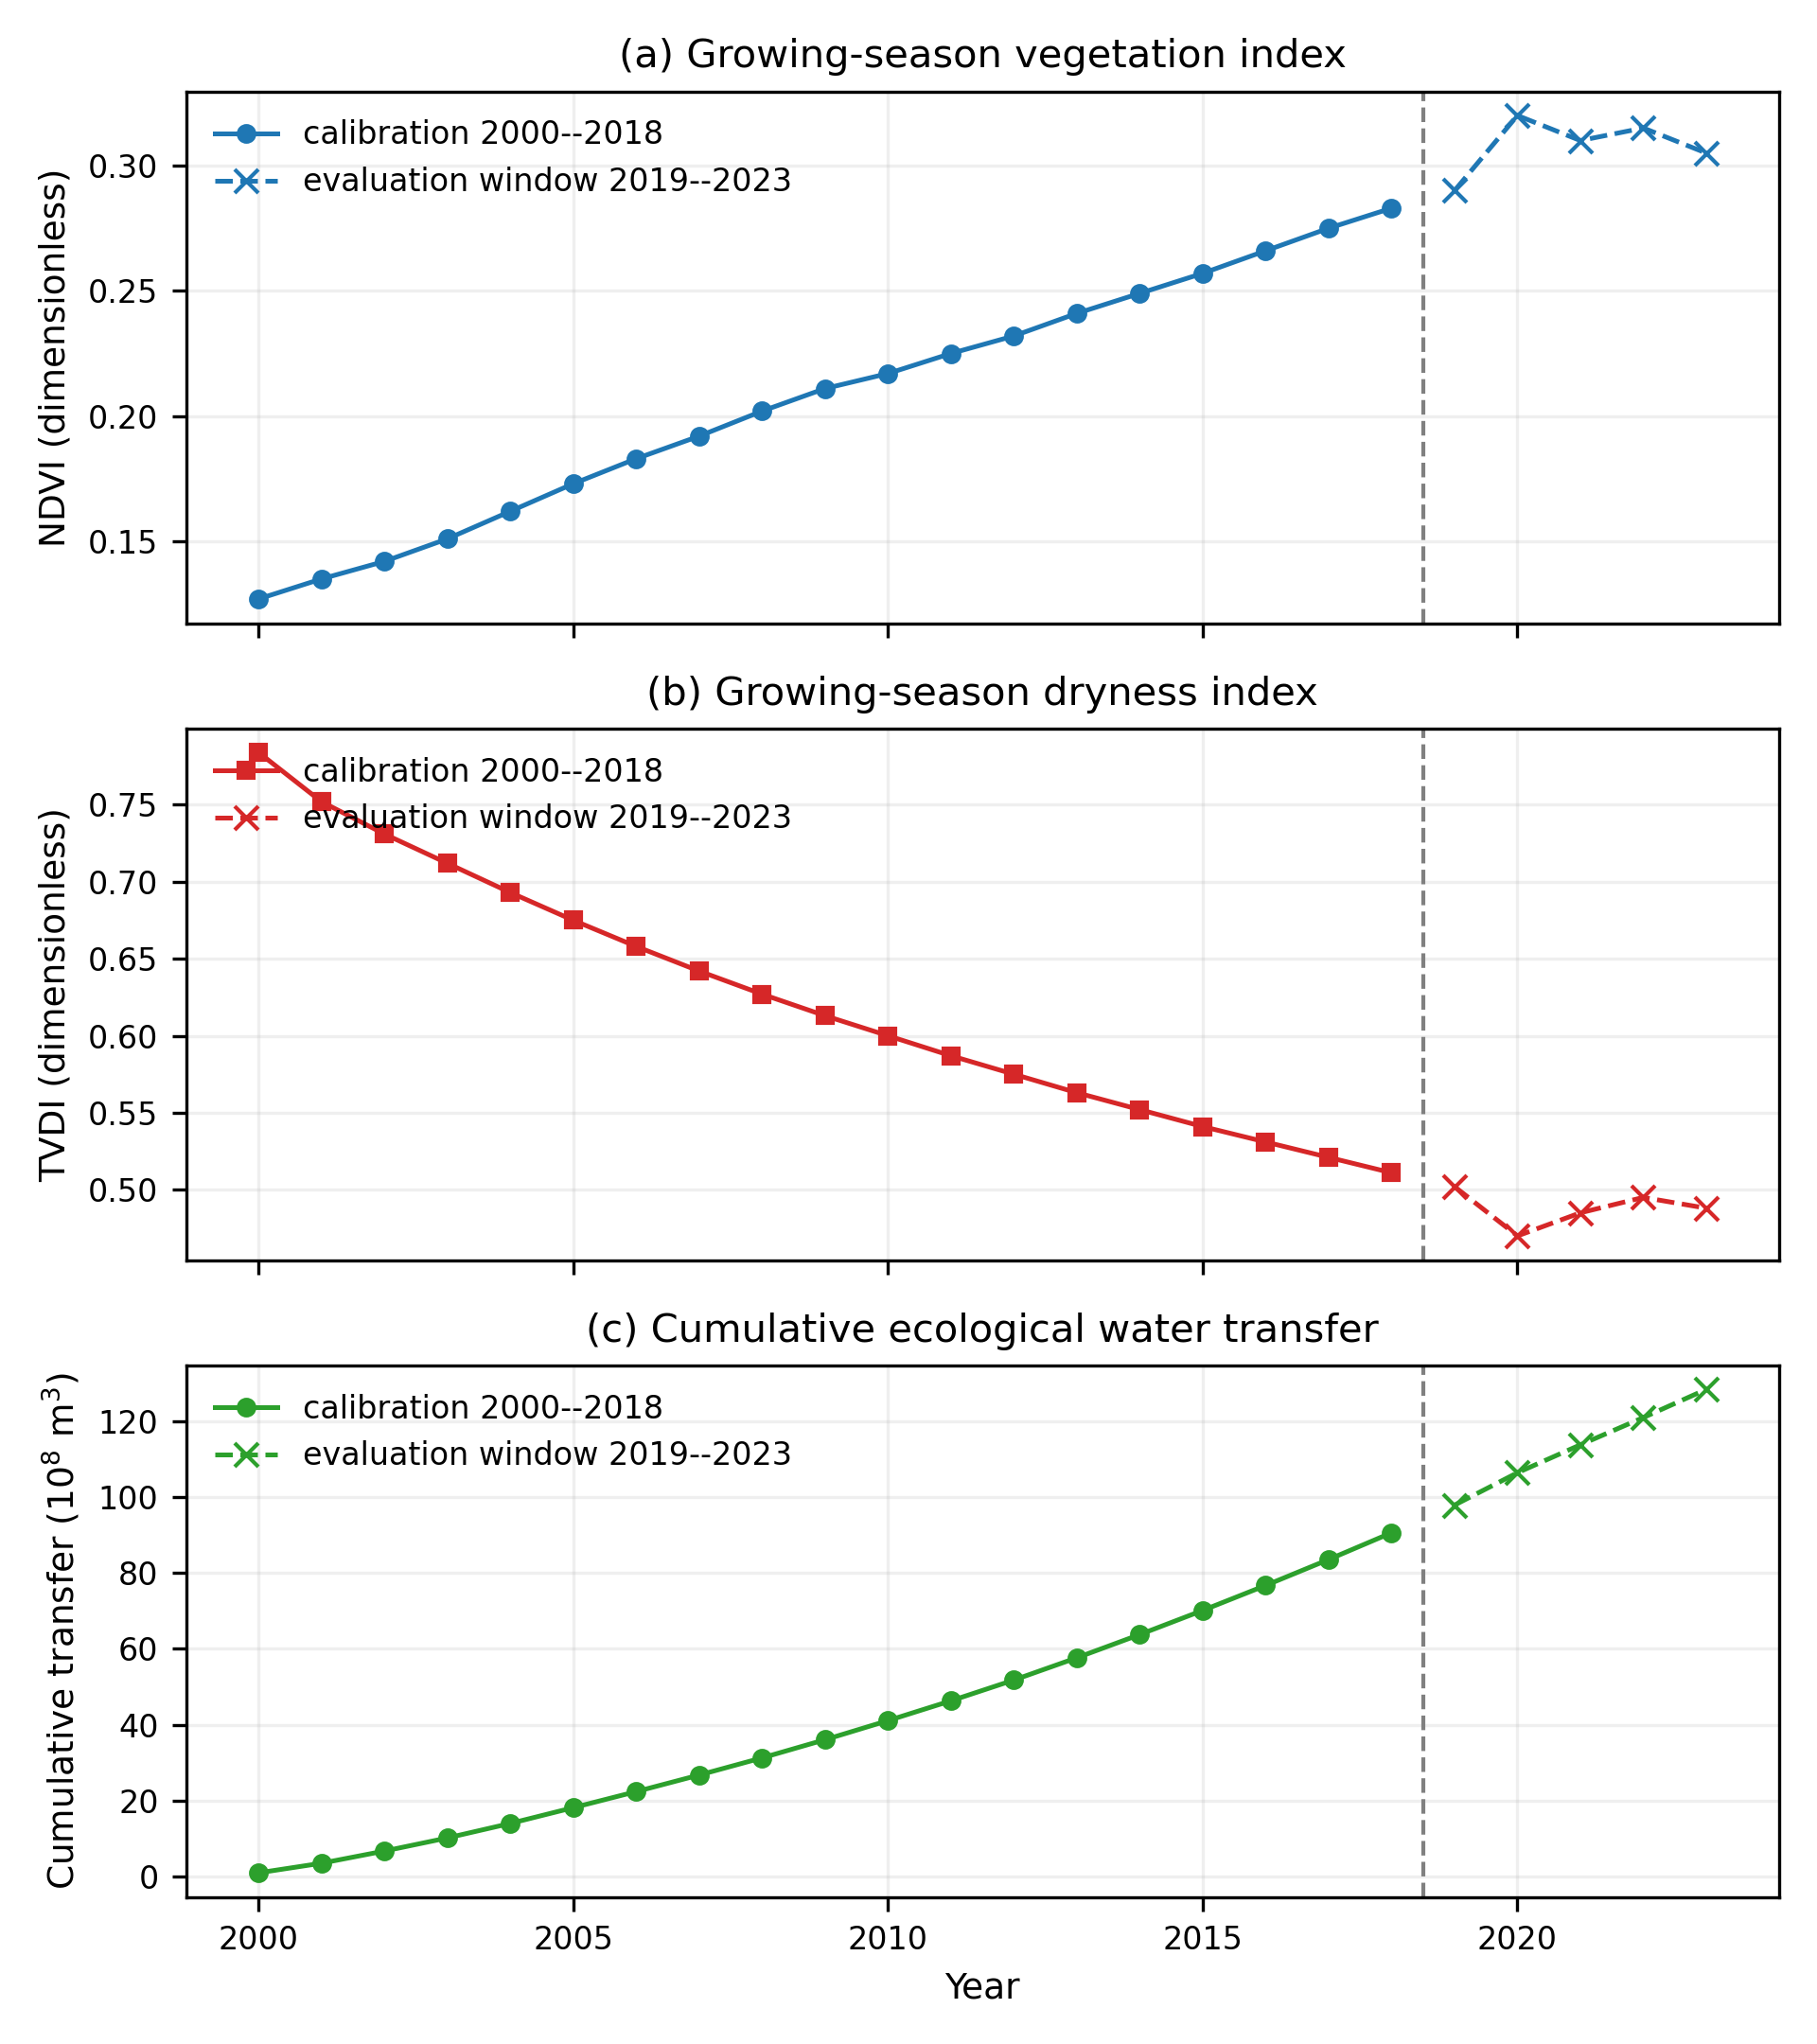
\includegraphics[width=0.80\textwidth]{fig1_observed_series.png}
	\caption{Observed annual series for the lower Tarim River (2000--2023), one variable per panel so that no two quantities share a vertical axis: (a) growing-season NDVI, (b) growing-season TVDI, and (c) cumulative ecological water transfer. Circles and solid lines mark the calibration period (2000--2018); crosses and dashed lines mark the evaluation window (2019--2023), which contains two withheld observations (2019--2020) and three trend-projected forcings (2021--2023). The evaluation entries lie outside the calibration range, so the right-hand part of each panel is an out-of-range transfer test rather than an interpolation check.}
	\label{fig:observed}
\end{figure}

\begin{figure}[H]
	\centering
	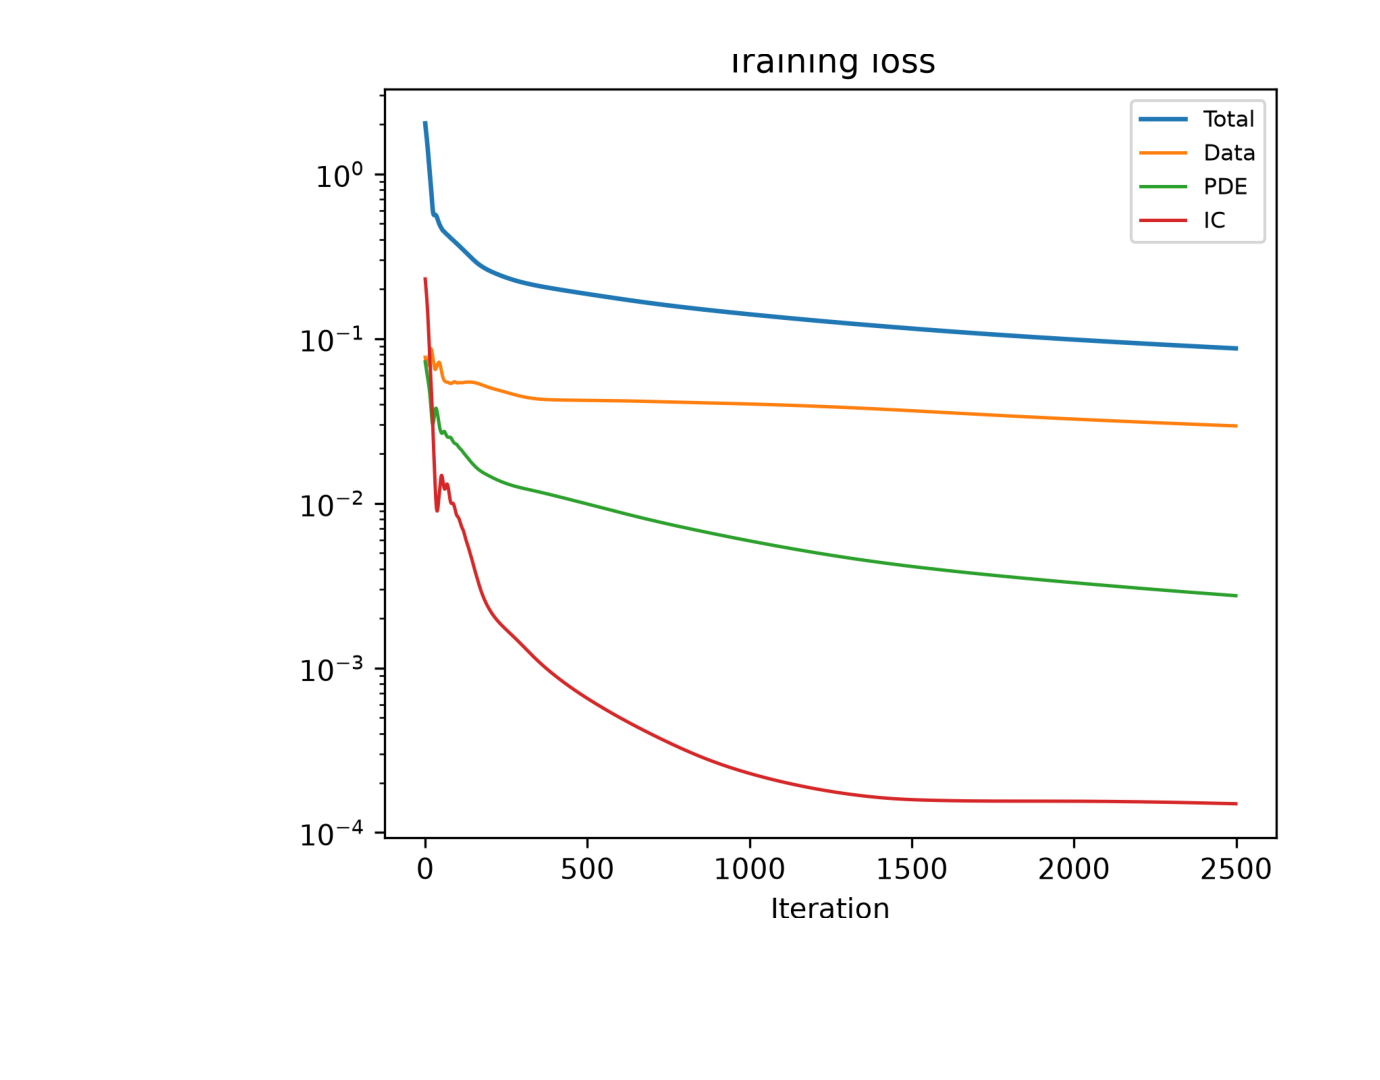
\includegraphics[width=0.60\textwidth]{fig_training_loss.png}
	\caption{Evolution of the loss components during PINN training.}
	\label{fig:loss}
\end{figure}

	The PINN provides point estimates for the normalized temporal-system parameters (Table~\ref{tab:params}). The main estimates are $a_1=0.705$, $a_2=0.570$, $a_3=0.322$, $a_4=0.567$, $b_1=0.129$, $b_2=0.017$, $b_3=0.252$ and $c_1=0.463$. Repeated refits with different random seeds reproduced the qualitative regime but moved the weakly identified coefficients $a_3$ and $b_2$ by more than an order of magnitude, so the values in Table~\ref{tab:params} are the archived set used for every downstream analysis and the sensitivity of the critical-point screen to this spread is audited in Supplementary Section~S7.
	
	\begin{table}[htbp]
		\centering
		\caption{Point estimates of the normalized ODE parameters obtained from PINN calibration.}
		\label{tab:params}
		\begin{tabular}{lcc}
			\toprule
			Parameter & Symbol & Estimated value \\
			\midrule
			Intrinsic vegetation response & $a_1$ & 0.705 \\
			Water contribution to vegetation & $a_2$ & 0.570 \\
			Vegetation--stress interaction & $a_3$ & 0.322 \\
			Vegetation loss rate & $a_4$ & 0.567 \\
			Stress generation & $b_1$ & 0.129 \\
			Water-related stress reduction & $b_2$ & 0.017 \\
			Stress relaxation & $b_3$ & 0.252 \\
			Water-input adjustment rate & $c_1$ & 0.463 \\
			\bottomrule
		\end{tabular}
	\end{table}
	
\subsection{Model Fit, Out-of-Range Extrapolation, and Model Comparison}
\label{subsec:validation}

\subsubsection{Reconstruction Performance}

The PINN achieved coefficients of determination of $R^2=0.993$ (NDVI), $R^2=0.996$ (TVDI) and $R^2=0.792$ (cumulative water transfer) over the calibration period 2000--2018 ($n=19$). In the original units the root-mean-square errors were 0.004 index units for NDVI, 0.005 index units for TVDI and $12.5\times10^{8}$ m$^{3}$ for cumulative water transfer. These values describe the reconstruction of the period used for calibration; over the complete 2000--2023 record the coefficients of determination are $0.944$, $0.976$ and $0.826$ for the three series.

\subsubsection{Out-of-Range Transfer: Withheld Observations and Projection Window}

The three series increase monotonically over the study period, so the evaluation values lie entirely outside the 2000--2018 calibration range (NDVI 0.290--0.320 versus 0.127--0.283; TVDI 0.470--0.502 versus 0.511--0.784; normalized cumulative water transfer 1.09--1.42 versus 0--1). This window therefore tests out-of-range transfer rather than interpolation, and it contains two different kinds of target. The 2019--2020 entries are withheld observations. The 2021--2023 entries are trend projections of the forcing series and are not independent validation data. The two are reported separately throughout.

Table~\ref{tab:holdout} reports the two windows separately. Within the calibration range the reconstruction tracks the observations closely. Outside it the model has no measurable skill: the coefficient of determination is negative for all three variables in both windows, and the error is larger than that of a persistence forecast. The largest relative error appears in the water-transfer state, which relaxes towards a forcing that leaves the calibration range.

\begin{table}[H]
	\centering
	\caption{Reconstruction and out-of-range transfer skill of the calibrated PINN. RMSE and MAE are reported in the original units of each variable (index units for NDVI and TVDI, $10^{8}$ m$^{3}$ for cumulative water transfer) and $R^2$ is computed on the same window as the error statistics. The 2019--2020 window contains two withheld observations and the 2021--2023 window contains three trend-projected entries; with so few points the coefficient of determination is unstable and should be read together with the error statistics.}
	\label{tab:holdout}
	\small
	\begin{tabular}{llcccc}
		\toprule
		Variable & Window & $n$ & $R^2$ & RMSE & MAE \\
		\midrule
		NDVI & Calibration 2000--2018 & 19 & 0.993 & 0.004 & 0.003 \\
		NDVI & Withheld observations 2019--2020 & 2 & $-3.45$ & 0.032 & 0.029 \\
		NDVI & Trend-projection window 2021--2023 & 3 & $-47.0$ & 0.028 & 0.028 \\
		TVDI & Calibration 2000--2018 & 19 & 0.996 & 0.005 & 0.004 \\
		TVDI & Withheld observations 2019--2020 & 2 & $-4.02$ & 0.036 & 0.033 \\
		TVDI & Trend-projection window 2021--2023 & 3 & $-30.5$ & 0.024 & 0.023 \\
		Water input & Calibration 2000--2018 & 19 & 0.792 & 12.51 & 10.78 \\
		Water input & Withheld observations 2019--2020 & 2 & $-12.6$ & 15.69 & 15.53 \\
		Water input & Trend-projection window 2021--2023 & 3 & $-26.0$ & 30.99 & 30.41 \\
		\bottomrule
	\end{tabular}
\end{table}

\subsubsection{Comparison with Baseline Models}

We compared the PINN against three reference models over the same windows: a persistence forecast that repeats the final calibration value, an AR(1) model fitted on 2000--2018 and then run in free simulation, and the same governing equations integrated forward with the PINN parameters. Table~\ref{tab:baseline} reports the RMSE in normalized units so that the three variables are directly comparable; the coefficient of determination is negative for every model in the evaluation window, so RMSE is used for the ranking.

\begin{table}[H]
	\centering
	\caption{RMSE comparison in normalized units over the calibration period and the combined evaluation window (2019--2023). Lower values are better. The AR(1) coefficients are estimated on the calibration window, so its calibration residual is zero by construction and is not a meaningful baseline for that window.}
	\label{tab:baseline}
	\small
	\begin{tabular}{lcccccc}
		\toprule
		& \multicolumn{3}{c}{Calibration 2000--2018} & \multicolumn{3}{c}{Evaluation 2019--2023} \\
		\cmidrule(lr){2-4} \cmidrule(lr){5-7}
		Model & NDVI & TVDI & Water & NDVI & TVDI & Water \\
		\midrule
		Persistence & 0.055 & 0.057 & 0.056 & 0.098 & 0.063 & 0.084 \\
		AR(1) free run & 0.000 & 0.000 & 0.000 & 0.082 & 0.069 & 0.012 \\
		Nonlinear ODE (forward) & 0.224 & 0.129 & 0.109 & 0.203 & 0.176 & 0.176 \\
		PINN & 0.026 & 0.018 & 0.140 & 0.190 & 0.107 & 0.290 \\
		\bottomrule
	\end{tabular}
\end{table}

Two points follow from Table~\ref{tab:baseline}. First, the PINN reconstructs the NDVI and TVDI series of the calibration period more accurately than either the forward-integrated ODE or the persistence forecast, while its water-transfer reconstruction is weaker than persistence because the water state relaxes towards the forcing rather than tracking it. Second, in the out-of-range window both mechanistic models are outperformed by the persistence and AR(1) forecasts. The governing-equation constraint therefore improves the description of the calibration period but does not extend the validity of the model beyond the range of the calibration data. This is the expected behaviour for a system that moves monotonically away from the calibration range, and it is the reason the present work is framed as parameter inversion and dynamical exploration rather than as forecasting.

\subsubsection{Ablation Study}

We also compared three loss configurations under an identical optimization budget: a data-only network, a network constrained by the governing-equation residual, and the full PINN with the initial-condition term added. The comparison is reported in Supplementary Section S7. All three configurations lose skill over the out-of-range window, and the data-only configuration attains a slightly lower average RMSE than the full PINN. The ablation therefore provides no evidence that the governing-equation residual improves out-of-range transfer for this dataset. Its role here is to constrain the parameter estimates and to keep the fitted trajectory dynamically consistent, not to improve extrapolation.

\subsubsection{Parameter Robustness}

	As a sensitivity check, 200 multiplicative perturbations drawn at $\pm10$, $\pm20$ and $\pm30\%$ were applied jointly to the eight parameters and the equilibrium branches were re-screened over the interval spanned by the observed normalized water input ($0.00$--$1.24$). No Hopf-type crossing appeared in any of the 600 perturbed sets, whereas fold-type crossings appeared in 0, 1 and 6 sets at $\pm10$, $\pm20$ and $\pm30\%$ respectively. The absence of a Hopf bifurcation is therefore robust to parameter perturbation in this range, while the absence of a fold point is conditional and becomes fragile once parameters move by more than about $20\%$. The scan and its output archive are described in Supplementary Section S7.

\subsection{Exploratory Hysteresis Scenario Based on PINN-Guided Normal Form}
\label{subsec:bifurcation}

To explore the potential for bistability and hysteresis within the parameter regime estimated by the PINN, we first analysed the full three-dimensional temporal ODE by treating the normalized ecological water input as a constant continuation parameter. The equilibrium structure of the original system was examined using a pseudo-arclength continuation implementation. Two continuation traces were obtained from the feasible equilibrium near the lower end of the investigated interval. The residuals of the continued equilibria were below $10^{-7}$, and local stability was evaluated from the eigenvalues of the full Jacobian matrix. No fold point satisfying the zero-eigenvalue and nondegeneracy criteria was identified, and no Hopf point satisfying the Routh--Hurwitz and transversality criteria was detected for the supplied PINN parameter set. The continuation result is shown in Fig.~\ref{fig:formal_continuation}. We therefore constructed a reduced cusp normal form anchored to the calibrated parameters only as a qualitative exploration of possible fold-like hysteresis, rather than as a direct bifurcation analysis of the original system.

\begin{figure}[H]
\centering
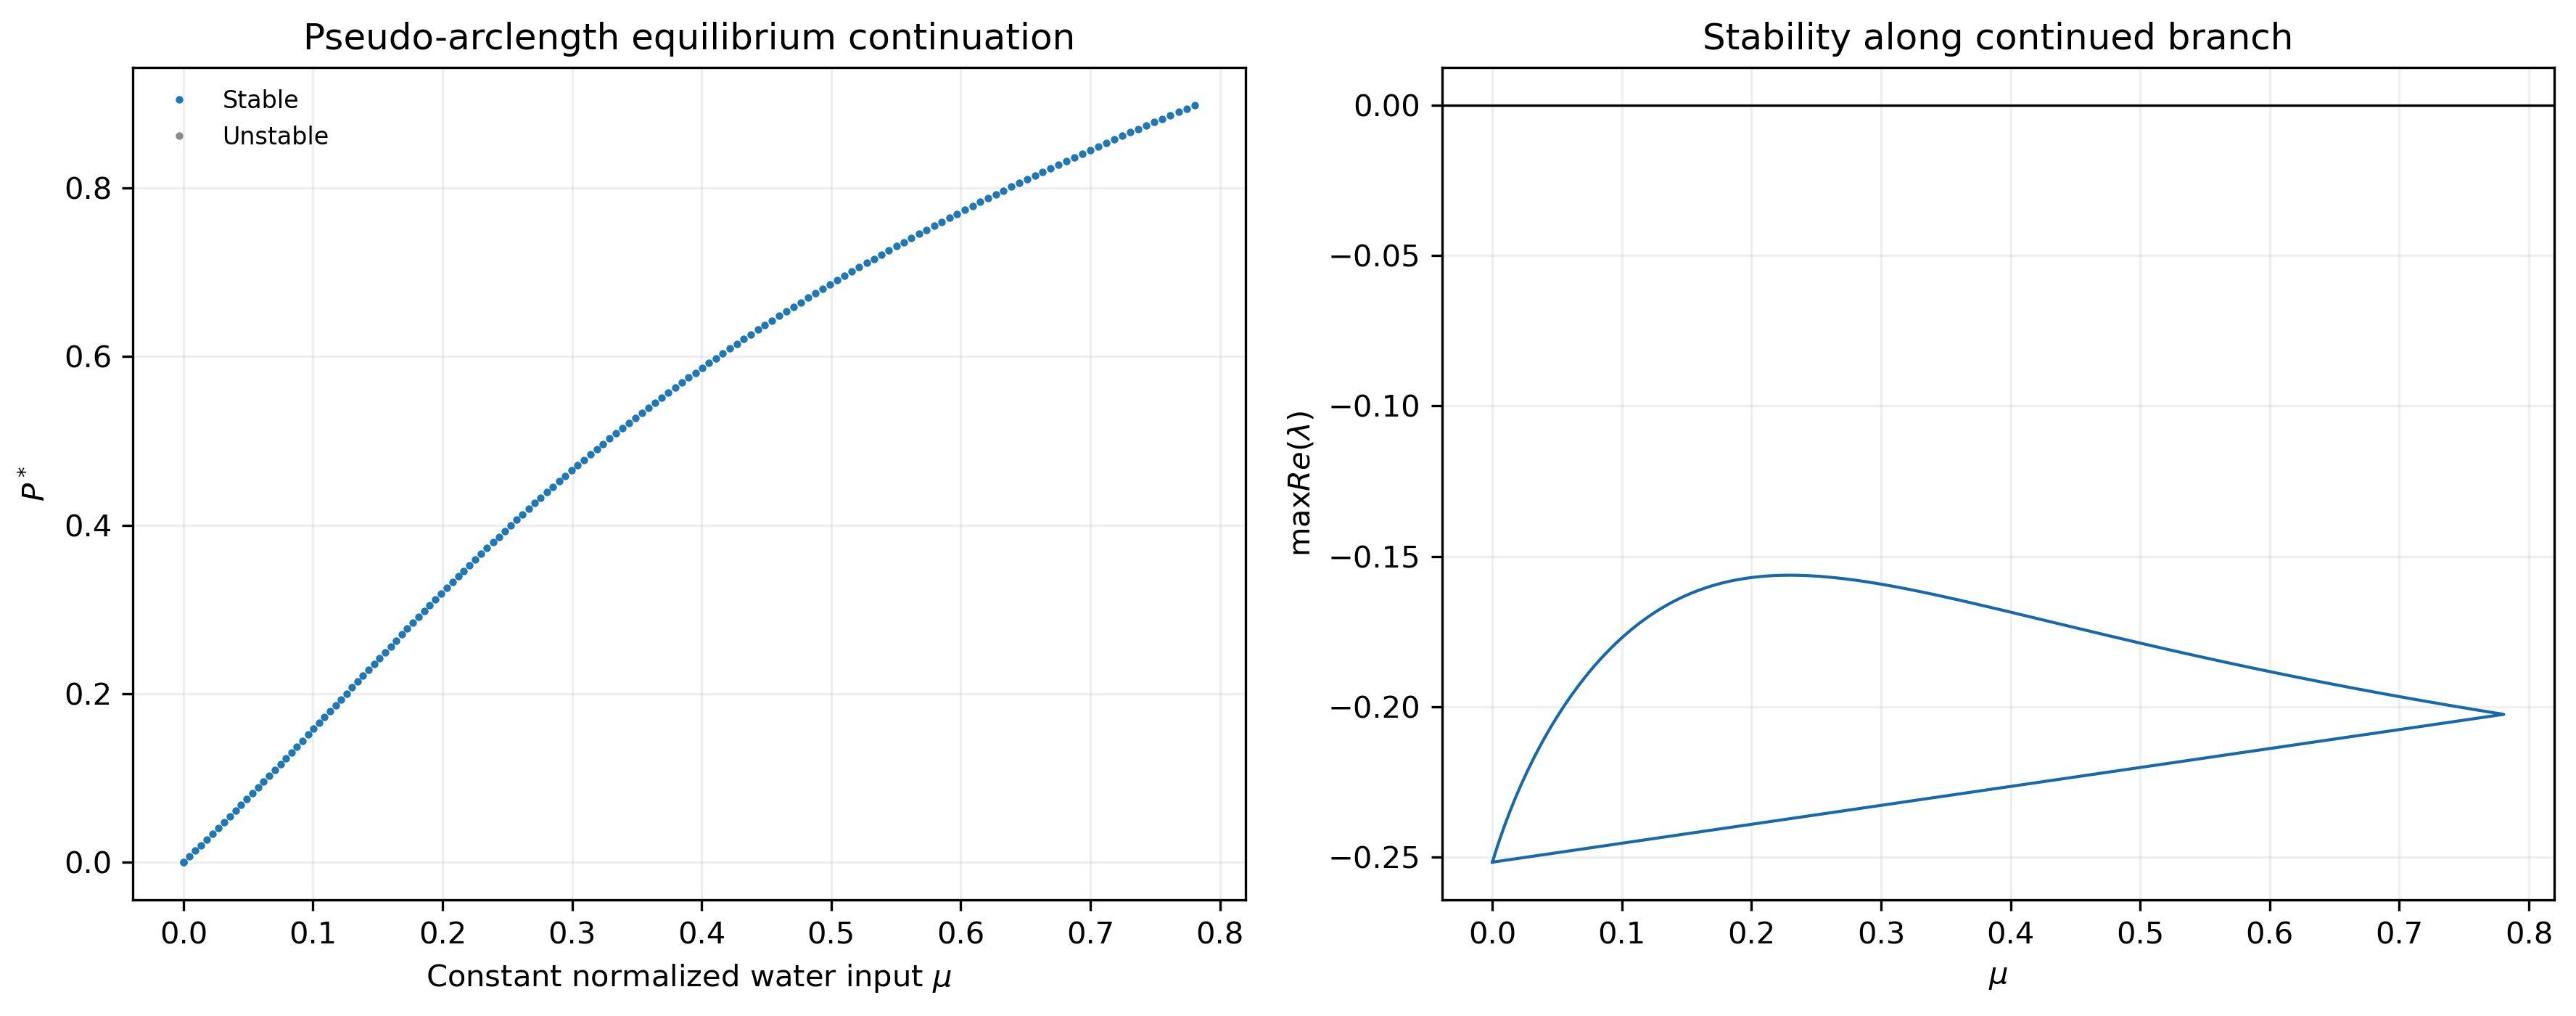
\includegraphics[width=0.98\textwidth]{fig_formal_continuation.png}
\caption{Full three-dimensional ODE equilibrium continuation and local stability analysis. Blue points indicate equilibria with negative real parts for all Jacobian eigenvalues. The maximum real eigenvalue remained negative along the computed traces, and no validated fold or Hopf point was detected for the supplied PINN parameter set.}
\label{fig:formal_continuation}
\end{figure}

	The resulting exploratory normal-form diagram is shown in Fig.~\ref{fig:bifurcation}. The diagram illustrates the qualitative possibility of alternative vegetation states and path dependence under changing water input. In the normalized water-input scale of the reduced normal form, the two exploratory turning points are approximately:

\begin{equation}
	F_{\mathrm{fold1}}^{\mathrm{(norm)}} \approx 0.35, \qquad 
	F_{\mathrm{fold2}}^{\mathrm{(norm)}} \approx 0.65,
	\label{eq:fold_normalized}
\end{equation}

The implied hysteresis width is approximately $\Delta F^{\mathrm{(norm)}} \approx 0.30$ in normalized model units.

The figure and the turning points use one coordinate system. The reduced normal form is
\begin{equation}
	\frac{\mathrm{d}x}{\mathrm{d}t} = -\left(x^{3} + a x + b\right), \qquad a = -3x_f^{2}, \qquad b = 2x_f^{3},
	\label{eq:normal_form}
\end{equation}
so that the folds sit at $x=\pm x_f$ with $x_f=0.5859$. Vegetation density is recovered as $P=(x+1)/2$, and the unfolding coordinate is mapped affinely onto the normalized water input, $F = 0.5 - s\,b$ with $s=(F_2-F_1)/4x_f^{3}$. With these constants the folds fall at $F_1=0.35$ ($P=0.793$) and $F_2=0.65$ ($P=0.207$). These are the values plotted in Fig.~\ref{fig:bifurcation}, reported in Eq.~(\ref{eq:fold_normalized}) and tabulated in Supplementary Section S4. The normal form is a qualitative device: it is not a continuation of the three-dimensional system, and the fold densities are chosen to bracket the vegetation range covered by the calibrated equilibrium branch.

\begin{figure}[H]
	\centering
	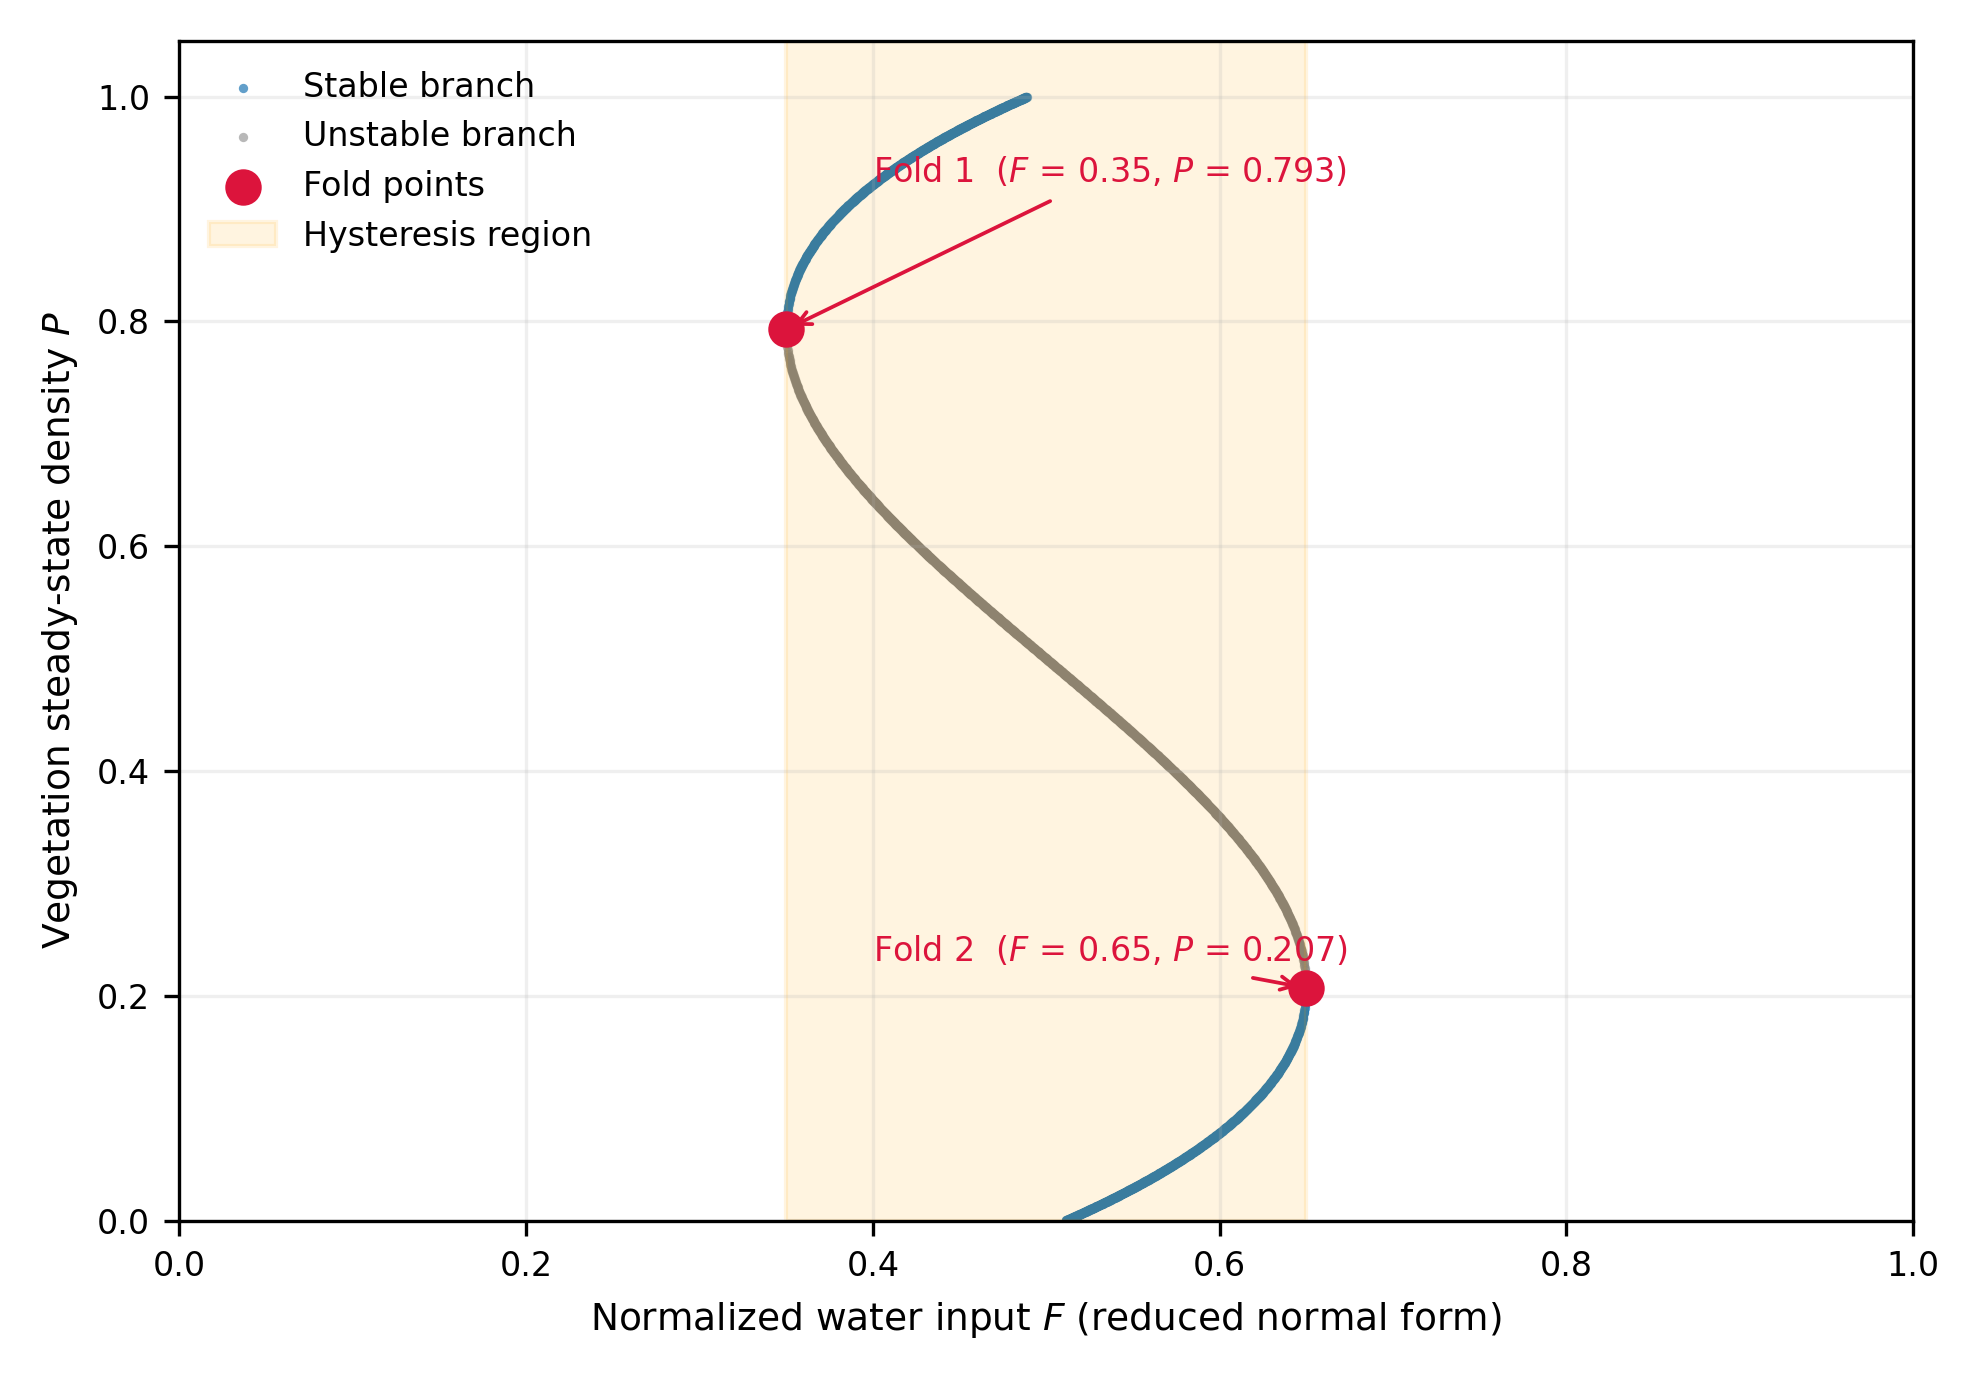
\includegraphics[width=0.8\textwidth]{fig9_bifurcation.png}
\caption{Exploratory hysteresis scenario generated by a reduced cusp normal form, plotted on the same normalized water-input scale $F$ used in Eq.~(\ref{eq:fold_normalized}). Blue marks the stable branch and grey the unstable branch, and the shaded band is the hysteresis region between the two fold points ($F=0.35$, $P=0.793$ and $F=0.65$, $P=0.207$). These values are scenario values of the reduced normal form and are not fold points of the full three-dimensional ODE.}
	\label{fig:bifurcation}
\end{figure}

	Under the supplied PINN parameter set and investigated normalized water-input interval, the full-system analysis did not provide evidence for a validated saddle-node/fold or Hopf bifurcation.
	
\subsection{Exploratory Turing Compatibility Test}
\label{subsec:turing}

To examine whether the PINN-estimated parameter regime is qualitatively compatible with spatial pattern formation, we conducted an exploratory Turing compatibility test using a separate reduced vegetation--water reaction--diffusion system. This system is a simplified mechanistic model based on classical pattern-formation theory \citep{turing1952chemical,rietkerk2008regular,meron2012pattern}:

\begin{equation}
	\left\{
	\begin{array}{rcl}
		\dfrac{\partial U}{\partial t} &=& r U (U - a)(1 - U) - m U V + D_u \nabla^2 U, \\[0.4cm]
		\dfrac{\partial V}{\partial t} &=& s - q V - c U V + D_v \nabla^2 V,
	\end{array}
	\right.
	\label{eq:turing_system}
\end{equation}

Here, \(U\) represents vegetation and \(V\) represents water/moisture. The parameters \(a\), \(D_u\), and \(D_v\) were not estimated by the PINN; instead, they were determined by a search procedure specifically designed to satisfy the classical linear Turing conditions. The complete derivation, parameter mapping, and search procedure are provided in Section S5 of the Supplementary Material.

	The corresponding characteristic wavelength is approximately \(\lambda = 2\pi/k_{\mathrm{peak}} \approx 4.19\) in model spatial units.

\begin{table}[htbp]
	\centering
	\caption{Results of the exploratory Turing compatibility test for the reduced vegetation--water verification system.}
	\label{tab:turing_results}
	\begin{tabular}{lcc}
		\toprule
		Quantity & Symbol & Value \\
		\midrule
		Vegetation equilibrium & $U^*$ & 0.645 \\
		Water equilibrium & $V^*$ & 0.688 \\
		Peak growth rate & $\sigma_{\max}$ & $1.51\times10^{-3}$ \\
		Peak wavenumber & $k_{\text{peak}}$ & 1.50 \\
		Pattern wavelength & $\lambda = 2\pi/k_{\text{peak}}$ & $\approx 4.19$ model units \\
		Classical Turing conditions in the reduced system & & Satisfied \\
		\bottomrule
	\end{tabular}
\end{table}

	Two checks are reported in Fig.~\ref{fig:turing}. First, the classical linear Turing conditions are satisfied for this parameter set, and the growth rate is positive over a broad band of wavenumbers, $0.06\le k\le 38.9$, with a maximum of $1.51\times10^{-3}$ at $k_{\mathrm{peak}}=1.50$. Second, a direct numerical integration of the same equations from a seeded perturbation reproduces the predicted growth rate to within 1\% ($1.52\times10^{-3}$ measured against $1.51\times10^{-3}$ analytic) and retains the seeded wavenumber. Because the unstable band is wide, the reduced system selects a wavelength only weakly; we therefore report the linear prediction and its numerical verification rather than presenting a saturated nonlinear pattern as an ecological prediction.

\begin{figure}[H]
	\centering
	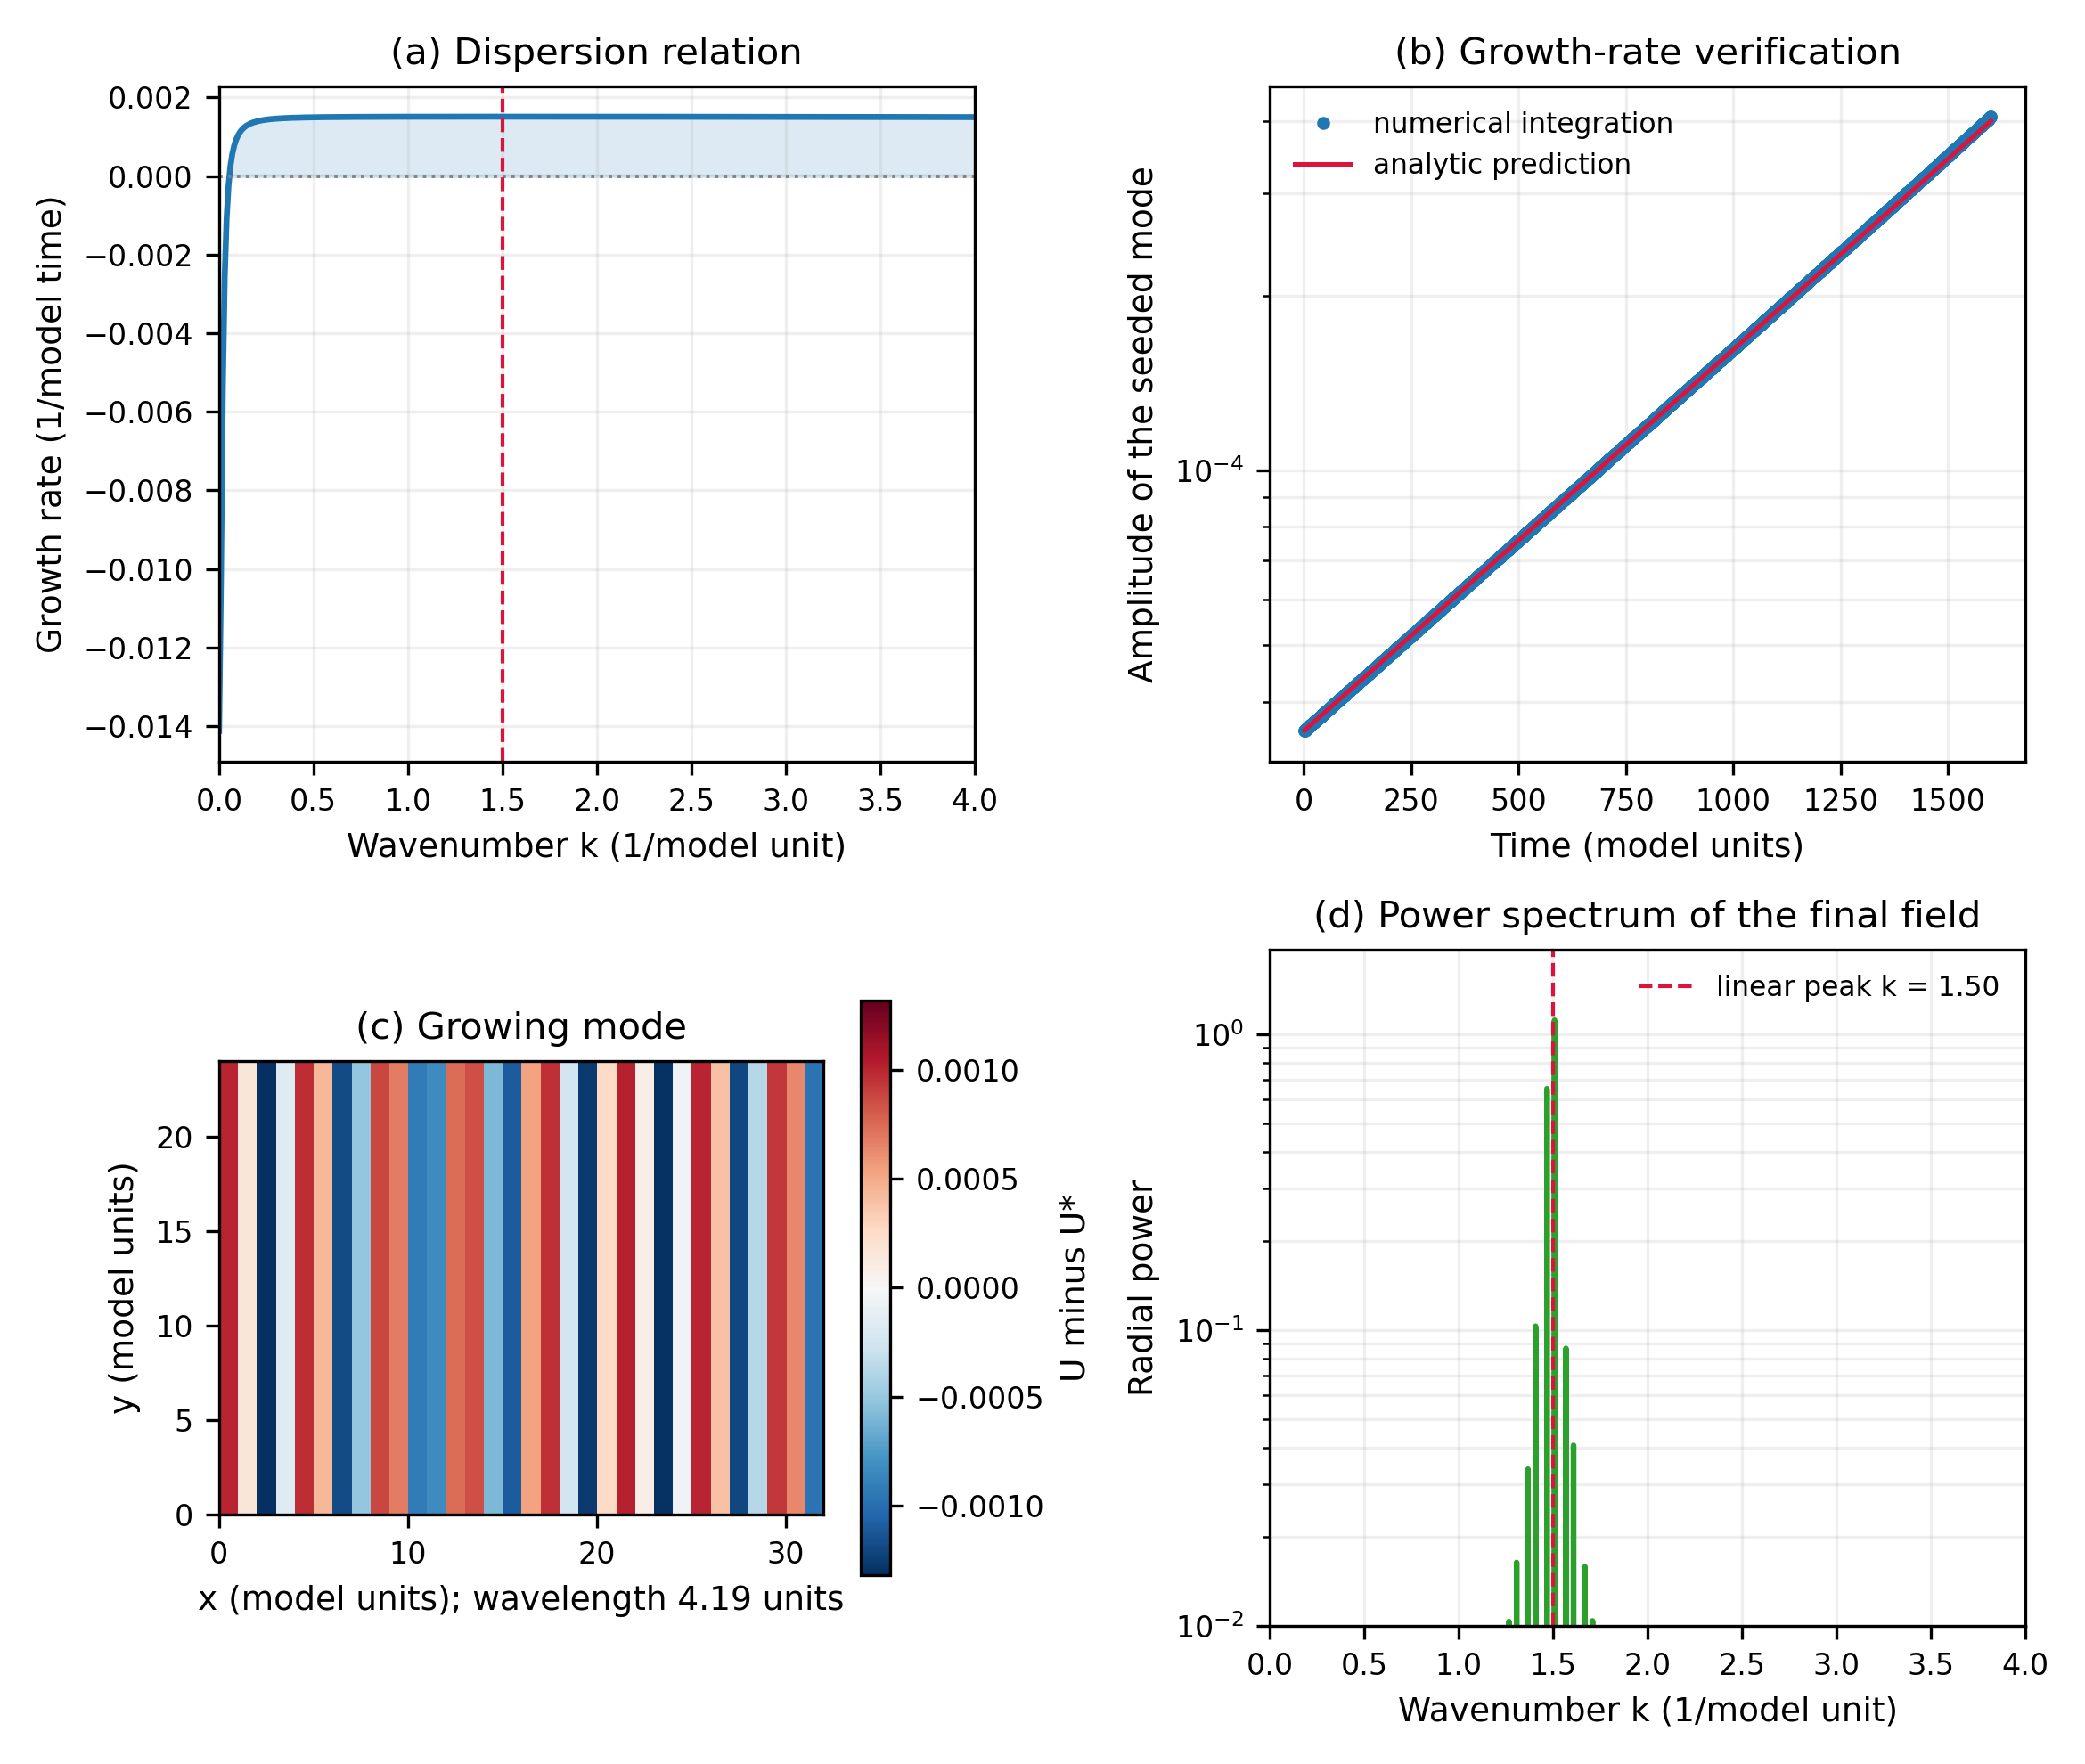
\includegraphics[width=0.8\textwidth]{fig17_turing_verification.png}
	\caption{Exploratory Turing compatibility test for the separate reduced reaction--diffusion system: (a) dispersion relation, where the growth rate is negative at $k=0$, positive over the band $0.06\le k\le 38.9$ and maximal at $k_{\mathrm{peak}}=1.50$ with $\sigma_{\max}=1.51\times10^{-3}$; (b) numerical integration of the seeded mode compared with the analytic exponential $\exp(\sigma_{\max}t)$, giving a measured slope of $1.52\times10^{-3}$; (c) spatial structure of the growing mode over a $32\times24$ model-unit window (wavelength $4.19$ units); (d) power spectrum of the final field, which remains concentrated at the seeded wavenumber. The analysis uses $U^{*}=0.645$, $V^{*}=0.688$, $a=0.295$, $D_u=10^{-6}$ and $D_v=10^{3}$ on a $128\times128$ lattice with spacing $\Delta x=1$. These parameters were selected by search rather than estimated by the PINN, and the figure verifies the linear prediction only; it is not a spatial calibration and no saturated nonlinear pattern is claimed.}
	\label{fig:turing}
\end{figure}

\begin{figure}[htbp]
	\centering
	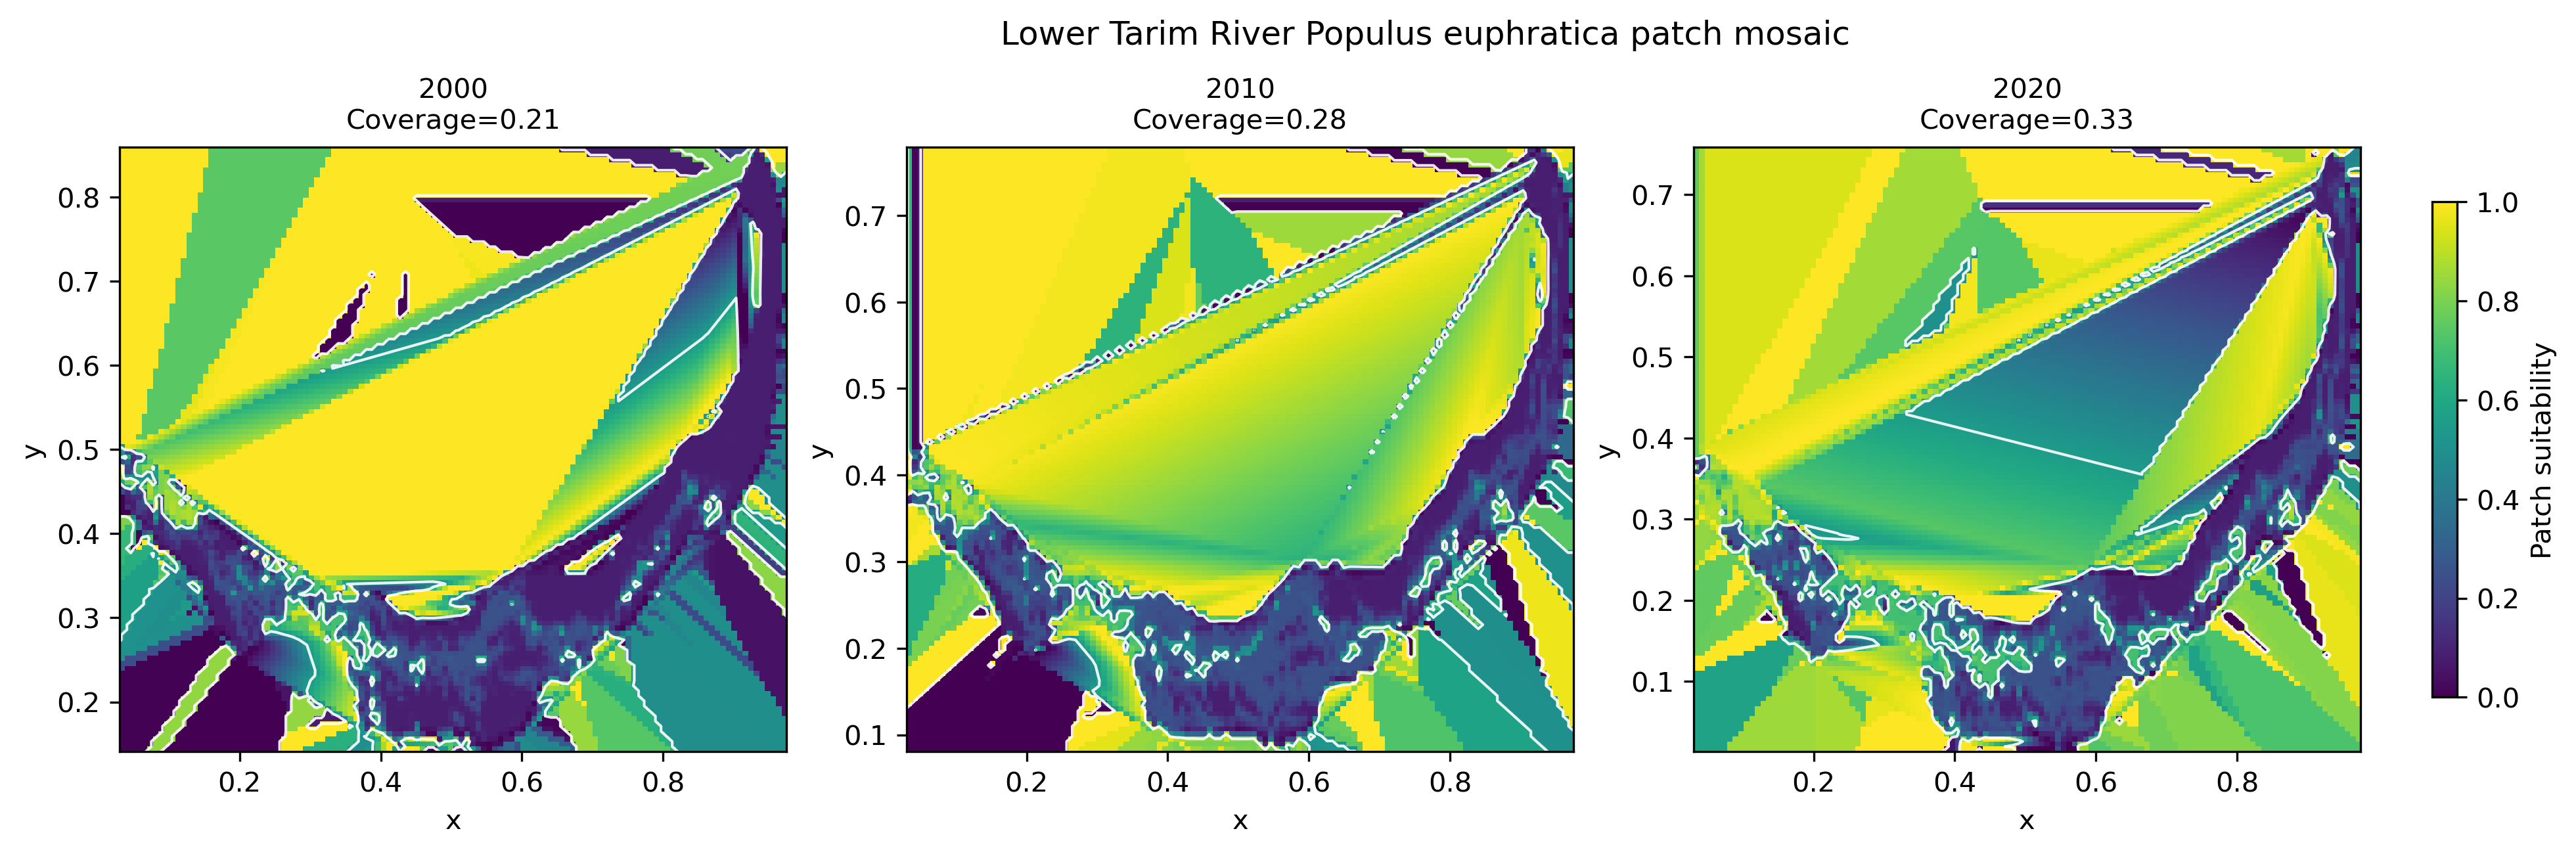
\includegraphics[width=0.85\textwidth]{fig15_tarim_patch_maps.png}
	\caption{Spatial distribution of vegetation patches from the Tarim River basin (qualitative reference).}
	\label{fig:patches}
\end{figure}

Additional spatial heatmaps, digitized literature-based spatial figures, and supplementary Tarim riparian patch maps are provided in Section S3 of the Supplementary Material.

\subsection{Held-out 10 m Pattern Test}
\label{subsec:spatial_pattern_results}

The unanchored spatial PINN fitted the calibration years but failed the temporal holdout: its mean $R^2$ across W1--W3 was negative for both $P$ and $R$ in 2022 and 2023 (from $-0.19$ to $-0.44$). Adding the 2021 persistence anchor removed this drift (Eq.~\ref{eq:spatial_pinn}). The anchored model reproduced the vegetation and water pattern structure, with a mean spectral cosine of $0.99$, a mean detrended pixel correlation of $0.94$ for $P$ and $0.90$--$0.92$ for $R$, and a random-phase null near $0.02$ (Table~\ref{tab:spatial_pattern}). The dominant $P/R$ wavelength matched the observed value in every window ($1122$, $281$ and $374$ m for W1--W3, a window mean of $592$ m).

\begin{table}[htbp]
	\centering
	\caption{Held-out pattern-level performance of the persistence-anchored residual spatial PINN on three 10 m windows. Values are means across W1--W3. The random-phase null is the pixel correlation obtained after randomizing the phase of the predicted field. Mean $P$ and $R$ pass the pre-specified criteria in both years; $P$ passes in all six window-years, whereas $R$ passes in four of six and fails the absolute-level criterion in W3. $T$ does not pass and is retained as a diagnostic state.}
	\label{tab:spatial_pattern}
	\begin{tabular}{lcccccc}
		\toprule
		Year & State & RMSE & $R^2$ & Spectral cosine & Pixel correlation & Null correlation \\
		\midrule
		2022 & $P$ & 0.075 & 0.903 & 0.992 & 0.942 & 0.019 \\
		2022 & $R$ & 0.132 & 0.601 & 0.987 & 0.903 & $-0.023$ \\
		2022 & $T$ & 0.265 & $-18.81$ & 0.978 & 0.556 & 0.021 \\
		2023 & $P$ & 0.085 & 0.875 & 0.986 & 0.944 & 0.018 \\
		2023 & $R$ & 0.138 & 0.629 & 0.989 & 0.920 & $-0.024$ \\
		2023 & $T$ & 0.371 & $-30.18$ & 0.936 & 0.465 & 0.011 \\
		\bottomrule
	\end{tabular}
\end{table}

The per-window check shows that $P$ passed in all six window-years. $R$ passed in four of six; the W3 window in 2022 and 2023 retained a pattern correlation above $0.80$ but failed the absolute-level criterion because of a large mean shift. This window is therefore reported as a pattern-level reconstruction rather than a validated absolute $R$ prediction. $T$ failed the absolute-level criterion in every window; its annual mean is controlled by interannual atmospheric and thermal conditions that are not represented by the current inputs. We therefore treat $T$ as a diagnostic state and do not use $T$ $R^2$ as a headline validation metric. The anchored model also remains slightly worse than one-year persistence in absolute 2023 $P$ and $R$ error, so the result supports pattern compatibility, not forecasting skill.
	\subsection{Consistency with Reported Ecosystem Conditions}

	The fitted temporal series is consistent with the observed ecological evolution of the lower Tarim River. The model reproduces the long-term increase in NDVI after the implementation of ecological water conveyance, while the TVDI trajectory reflects a general reduction in vegetation water stress. The inferred water-input series also follows the temporal variation of the reported ecological water-conveyance records.

	The spatial analysis provides a bounded consistency check. The reduced reaction--diffusion system admits a Turing-unstable band of wavenumbers with a characteristic wavelength of a few model units, which is qualitatively compatible with the spatial heterogeneity reported for the Tarim River riparian ecosystem \citep{ma2025response}. The separate 10 m test adds a data-facing check: the anchored residual PINN reproduces the held-out vegetation and water pattern structure and its dominant wavelength, while the unanchored control does not. Because the 10 m test covers three local windows, does not recover the W3 water-level shift, and does not predict the absolute TVDI level, it supports pattern compatibility rather than a basin-wide spatial prediction.
	\subsection{Descriptive Cross-Basin Comparison}
	\label{subsec:cross_basin}

	To provide a descriptive cross-basin comparison, we repeated the remote-sensing processing for the lower Heihe (Ejina Oasis) using the same MODIS products.

	Using point-consistent annual summaries, lower Tarim NDVI increased from 0.0758 in 2000 to 0.1141 in 2023 (+50.5\%, trend $+0.0017$ yr$^{-1}$, $R^2=0.797$). Lower Heihe NDVI increased from 0.1322 to 0.1446 over the same period (+9.4\%, trend $+0.0008$ yr$^{-1}$, $R^2=0.652$). The lower Heihe series therefore shows a weaker but still positive vegetation signal. Mean Ejina TVDI over 2000--2023 was 0.696, with an annual range of 0.663--0.736.

	The Zhengyixia hydrological record contains a sourced annual release value for 11 of 24 water years. Across these 11 available years, NDVI and water release had a positive association ($r=0.55$). Missing water years were retained as missing.

	\begin{figure}[htbp]
		\centering
		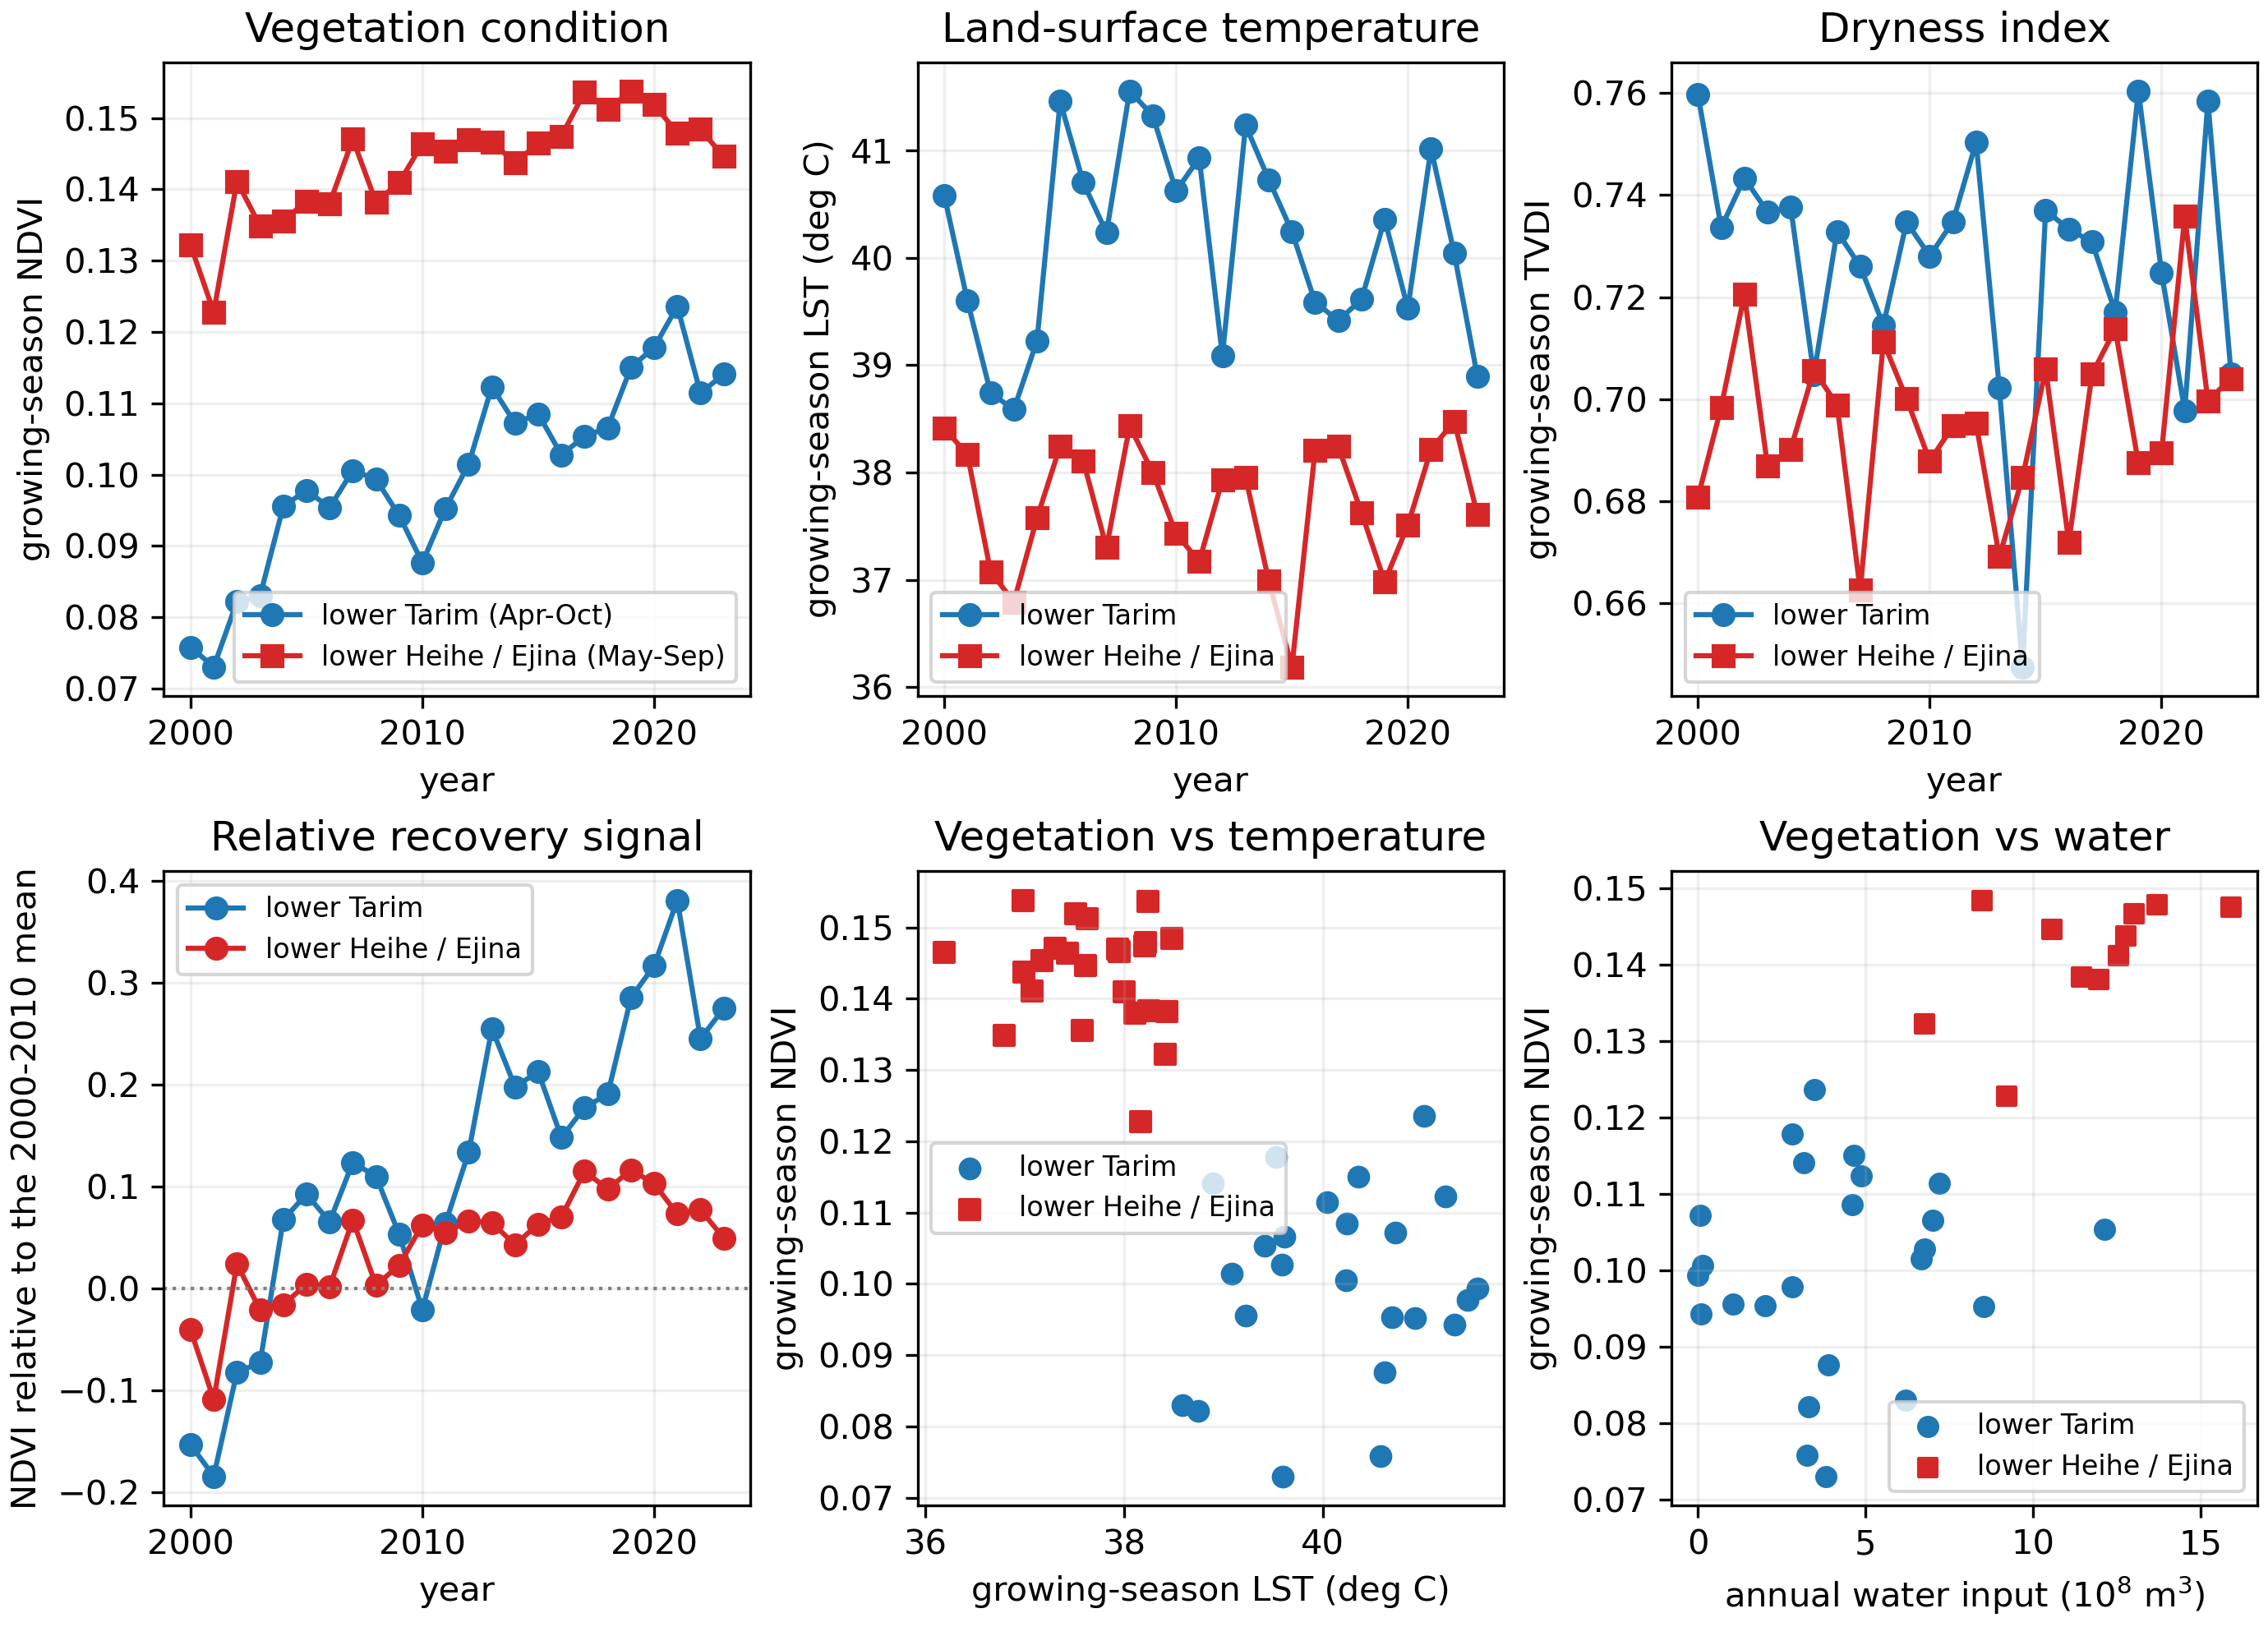
\includegraphics[width=\textwidth]{fig_cross_basin_trends.png}
		\caption{Descriptive cross-basin comparison of the lower Tarim River corridor and the lower Heihe (Ejina Oasis). The Ejina series use the point-consistent annual summaries; TVDI is an empirical MODIS-based dryness index. The lower Heihe water record is available for only 11 of 24 water years.}
		\label{fig:cross_basin}
	\end{figure}

	\begin{table}[H]
		\centering
		\caption{Descriptive cross-basin summary for 2000--2023. Ejina values use the point-consistent annual sample; Tarim values use the 1 km river-corridor series.}
		\label{tab:cross_basin}
		\small
		\begin{tabular}{@{}lrrrrrr@{}}
			\toprule
			Basin & \multicolumn{2}{c}{NDVI} & Change & NDVI trend & TVDI & Water \\
			\cmidrule(lr){2-3}
			 & 2000 & 2023 & (\%) & (yr$^{-1}$) & mean & years \\
			\midrule
			Lower Tarim & 0.0758 & 0.1141 & +50.5 & +0.0017 & 0.727 & 21+3/24 \\
			Lower Heihe (Ejina) & 0.1322 & 0.1446 & +9.4 & +0.0008 & 0.696 & 11/24 \\
			\bottomrule
		\end{tabular}
		\caption*{Note: The cross-basin comparison is descriptive. Ejina TVDI is an empirical NDVI--LST feature-space index, not a ground measurement; dry-edge $R^2$ was below 0.10 in 2000, 2003, 2013 and 2022. The Tarim water count denotes 21 reported or compiled values plus three trend projections; the lower Heihe count denotes 11 available Zhengyixia annual release values.}
	\end{table}

	% ==================== 4. Discussion ====================
	\section{Discussion}
	
	\subsection{Ecological Implications}
	
	The reduced reaction--diffusion verification is an \emph{exploratory compatibility test}. It shows that the selected reduced system satisfies the classical linear Turing conditions, that its unstable band is broad, and that the predicted growth rate is reproduced by direct numerical integration. The characteristic wavelength at the band maximum is approximately \(\lambda\approx4.19\) in model spatial units, but the flatness of the dispersion relation means that no single wavelength is sharply selected, so the result supports compatibility with patterned vegetation rather than a specific predicted pattern.

	\subsection{Cross-Basin Interpretation}

	Processing the lower Heihe with the same MODIS workflow lets the Tarim result be read against a second endorheic riparian system instead of in isolation. Both basins gained greenness over 2000--2023, but the Tarim corridor change (+50.5\%, $+0.0017$ yr$^{-1}$, $R^2=0.797$) is roughly five times the Ejina change (+9.4\%, $+0.0008$ yr$^{-1}$, $R^2=0.652$), and mean Ejina TVDI (0.696) indicates slightly less growing-season dryness than the Tarim corridor (0.727). Two readings of that contrast are compatible with the present data. Either the Tarim recovery is genuinely further along its response to two decades of concentrated conveyance, or the Ejina vegetation is closer to a moisture-limited ceiling so that additional water produces a smaller marginal greenness gain. The available record cannot separate these readings, because the Ejina water forcing is only partial: Zhengyixia release is documented for 11 of 24 water years, whereas the Tarim series is near-complete (21 compiled values plus three trend projections). The positive but modest association between release and NDVI across the 11 Ejina water years ($r=0.55$) is consistent with a weaker forcing--response coupling, but with this sample size it is also consistent with a moderate coupling measured noisily.

	The practical consequence is that the calibrated Tarim parameters should be treated as basin-specific. The cross-basin comparison is a descriptive reference for interpreting the Tarim trajectory, not a transferability test, and the Ejina series was never used to calibrate or validate the Tarim PINN. A genuine two-basin test would require a complete multi-year Heihe release record, ideally with East Juyan Lake inflow as an independent check on the Zhengyixia series, and a separate calibration of the same model form on that record so that the two parameter sets could be compared directly.
	
	\subsection{Management Implications}
	
	Based on the model results, we recommend:
	\begin{enumerate}
		\item Implement concentrated ecological water releases during May--July, which corresponds to the main period of ecological water demand in the lower Tarim River \citep{ye2010ecological}.
		\item Enhance vegetation--water feedbacks through soil organic matter management and mulching. This maps to increasing the water-contribution parameter \(a_2\) and reducing the stress-interaction parameter \(a_3\) through improved moisture retention and reduced evaporative stress.
		\item Monitor early warning signals (critical slowing down, increased variance) to detect impending state shifts. The early warning analysis is presented in Supplementary Section S3.1.
	\end{enumerate}
	
	\subsection{Model Limitations}
	
Several limitations should be acknowledged: (i) the model treats vegetation as a single state variable, neglecting age structure and species composition; (ii) groundwater dynamics and climate covariates are not explicitly modelled; (iii) the annual record is short, the evaluation values lie outside the calibration range and only two of them are withheld observations, so the reported scores quantify out-of-range transfer rather than interpolation accuracy, and the model is not presented as a forecasting tool; (iv) the temporal calibration uses reach-scale annual aggregates of a single river reach, whereas the 10 m pattern test covers only three local windows, so neither dataset provides plot-level or basin-wide spatial calibration; (v) the lower Heihe comparison is descriptive, a sourced water-release value exists for only 11 of 24 years, and the basin is not an independent calibration or validation of the Tarim PINN; (vi) repeated refits with different random seeds reached the same qualitative parameter regime but varied the weakly identified coefficients by up to an order of magnitude, so the archived parameter set used for the downstream analyses should be read together with the perturbation audit in Section S7, and a version-pinned, fixed-seed re-run is required before release; (vii) the Turing verification uses a simplified system with search-selected parameters and no georeferenced spatial calibration; and (viii) the spatial pattern test excludes 2015, treats 2016 top-of-atmosphere data as low-reliability, does not recover the W3 water-level shift, and cannot predict the absolute TVDI level, so it supports pattern-level compatibility rather than spatial forecasting.
	
	% ==================== 5. Conclusion ====================
\section{Conclusion}

	This study developed a time-dependent PINN-constrained framework for parameter inversion and dynamical exploration of vegetation--water dynamics in the lower Tarim River. The PINN reproduced the calibration-period NDVI, TVDI and cumulative water-transfer series with coefficients of determination of 0.993, 0.996 and 0.792, but it has no measurable skill outside the calibration range, where a persistence forecast is more accurate. The evaluation is therefore reported in three separate windows: calibration (2000--2018), two withheld observations (2019--2020) and three trend-projected years (2021--2023).

	A separate persistence-anchored residual spatial PINN reproduced the 2022--2023 vegetation and water pattern structure on three georeferenced 10 m windows (mean spectral cosine $\approx0.99$; mean pixel correlation $0.90$--$0.94$), while the unanchored spatial model did not. The anchored model did not improve the absolute 2023 level relative to one-year persistence, did not recover the W3 water-level shift, and did not predict the absolute TVDI level. The spatial result therefore supports pattern-level compatibility, not spatial forecasting.

The calibrated parameters support equilibrium and stability analysis of the full three-dimensional ODE, while the reduced normal-form and Turing analyses provide exploratory tests of qualitative hysteresis and spatial-pattern compatibility. The full-system continuation analysis did not provide evidence for a validated saddle-node or Hopf bifurcation under the supplied calibrated parameter set and the investigated water-input range, and the reduced normal-form diagram is a qualitative illustration rather than a bifurcation result of the calibrated three-dimensional ODE. A descriptive comparison with the lower Heihe (Ejina Oasis), processed with the same remote-sensing workflow, shows a weaker but still positive vegetation signal; the two basins differ in both trend magnitude and water-record availability, so that comparison remains descriptive. Future work should incorporate longer records, groundwater observations, repeated temporal validation with genuinely withheld years, version-pinned PINN restarts, basin-wide georeferenced rasters and atmospheric covariates for the TVDI state.
	
	% ==================== 6. Supplementary Materials ====================
	\section*{Supplementary Materials}
	
	The supplementary material associated with this article includes:
	\begin{itemize}
		\item \textbf{Section S1:} Mathematical analysis of the calibrated temporal
		ODE, including the Jacobian matrix and bifurcation conditions.
		
		\item \textbf{Section S2:} PINN architecture, loss function, and training
		hyperparameters.
		
		\item \textbf{Section S3:} Supplementary results, including early-warning
		analysis, scenario analysis, correlation analysis, and spatial pattern
		visualization.
		
		\item \textbf{Section S4:} Exploratory reduced-model bifurcation and
		sensitivity analysis.
		
		\item \textbf{Section S5:} Turing verification of the separate reduced
		reaction--diffusion system.
		
		\item \textbf{Section S6:} Data tables and preprocessing methods for NDVI,
		TVDI and ecological water input, including the lower Heihe cross-basin
		comparison, annual TVDI edge diagnostics and archived Heihe water records.
		\item \textbf{Section S7:} Additional details on baseline models, ablation study, and parameter robustness analysis.
	\item \textbf{Section S8:} Documentation of the 10 m spatial pattern test, including the window inventory, validity screen, holdout protocol and per-window results.
		\item Annual water-transfer, NDVI and TVDI data tables with reliability labels.
	\end{itemize}
	
	
	% ==================== CRediT ====================
	\section*{CRediT authorship contribution statement}
	\textbf{Yingxin Pang:} Conceptualization, Methodology, Software, Formal analysis, Investigation, Data Curation, Writing -- Original Draft, Visualization, Validation.
	
	\textbf{Jinhua Zhang:} Software, Formal analysis, Data Curation, Writing -- Review \& Editing, Visualization.
	
	\textbf{Jianwei Shen:} Conceptualization, Methodology, Resources, Writing -- Review \& Editing, Supervision, Project Administration, Funding Acquisition.
	
	
	\section*{Declaration of competing interest}
	The authors declare that they have no known competing financial interests or personal relationships that could have appeared to influence the work reported in this paper.
	
	
	\section*{Acknowledgements}
	This work was supported by the National Natural Science Foundation of China (Grant No. 12272135); the Natural Science Foundation of Henan Province, China (Grant No. 262300421368); and the Henan Province Science and Technology Research Project (Grant No. 262102240082).
	
	
\section*{Data Availability Statement}

Processed annual NDVI and TVDI series, TVDI edge diagnostics, point audits,
compiled water tables, spatial-window model outputs, analysis code, and figure
files are openly available in the \href{https://github.com/PangYingxin-max/lower-tarim-pinn/tree/v1.0.1}{GitHub repository snapshot v1.0.1}.
The repository also provides the Google Earth Engine scripts and source URLs
for the satellite products. Raw MODIS, Sentinel-2, and Landsat scenes are not
redistributed. Tarim water entries for 2021--2023 include report-based or
derived values, and the Heihe Zhengyixia release series contains 11 of 24 water
years; these limitations and row-level sources are documented in the
repository.
	
	
	\section*{Declaration of Generative AI and AI-assisted technologies in the writing process}
	ChatGPT (OpenAI) was employed during the manuscript preparation phase to assist with language polishing and grammatical verification. The authors have taken full accountability for the content, following comprehensive review and necessary editing of the AI-generated suggestions.
	
	
	\bibliographystyle{elsarticle-num}
\bibliography{myrefs}
	
\end{document}
